\documentclass[times,10pt,twocolumn]{article} 

%% Nous avons déjà sélectionné quelques packages, si vous avez besoin
%% d'ajouter un nouveau package, veuillez contacter l'équipe (actes
%% (AT) lists.sstic.org) car nous devons vérifier la compatibilité des
%% modules entre eux.
%% 
\documentclass[times,10pt,twocolumn]{article} 

%% Nous avons déjà sélectionné quelques packages, si vous avez besoin
%% d'ajouter un nouveau package, veuillez contacter l'équipe (actes
%% (AT) lists.sstic.org) car nous devons vérifier la compatibilité des
%% modules entre eux.
%% 

\makeindex
\usepackage{latex8}
\usepackage{amssymb}
\usepackage{graphicx}
\usepackage{xcolor}
\usepackage[utf8x]{inputenc}
\usepackage{url}
% \usepackage{url,hyperref}
% \usepackage{float}

% \usepackage{url}
% \usepackage{array}
% \usepackage{fullpage}
% \usepackage{float}
% \usepackage{framed}
% \usepackage{francais}

% \usepackage{wrapfig}

\usepackage{wrapfig}

% \usepackage[french]{babel}
% \usepackage[utf8x]{inputenc}
% \usepackage[fit]{truncate}
% \usepackage{xspace}
% \usepackage{xcolor}
% \usepackage{graphicx}
% \usepackage{fancyhdr}
\usepackage{listings}
% \usepackage{ifthen}
% \usepackage{url}

\usepackage{makeidx}
% \makeindex

\usepackage[T1]{fontenc}
\usepackage{tabularx}
\usepackage{array}
\usepackage{multirow}
\usepackage{lscape}
% \usepackage{fancyhdr}
\pagestyle{empty}
% \cfoot{}

\makeatletter
\def\and{%
  \end{tabular}%
  \hskip 0.1em \@plus.17fil\relax
  \begin{tabular}[t]{c}}
\makeatother

% \documentclass[times,11pt,fullpage]{article}

% \usepackage{amssymb} % not included
% \usepackage{graphicx} % included
% \usepackage[utf8x]{inputenc} % not included
% \usepackage{url,hyperref} % not included
% \usepackage{fullpage} % not included
% \usepackage{float} %not included
% \usepackage{framed} %not included
% \usepackage{francais} %included
% \usepackage{wrapfig} %not included

%%%% debut macro %%%%
\newenvironment{changemargin}[2]{\begin{list}{}{%
\setlength{\topsep}{0pt}%
\setlength{\leftmargin}{0pt}%
\setlength{\rightmargin}{0pt}%
\setlength{\listparindent}{\parindent}%
\setlength{\itemindent}{\parindent}%
\setlength{\parsep}{0pt plus 1pt}%
\addtolength{\leftmargin}{#1}%
\addtolength{\rightmargin}{#2}%
}\item }{\end{list}}
%%%% fin macro %%%%

% Duqu modules
\newcommand{\Crysys}{\texttt{CrySys}}
\newcommand{\Duqu}{\texttt{Duqu}}
\newcommand{\Stuxnet}{\texttt{Stuxnet}}
\newcommand{\driver}{\texttt{nfrd965.sys}}
\newcommand{\netpDLL}{\texttt{NETP191.PNF}}
\newcommand{\cmiDLL}{\texttt{CMI4432.PNF}}
\newcommand{\netpCONF}{\texttt{netp192.PNF}}
\newcommand{\cmiCONF}{\texttt{CMI4464.PNF}}
\newcommand{\jminet}{\texttt{JMINET7.SYS}}
\newcommand{\cmi}{\texttt{CMI4432.SYS}}
\newcommand{\krn}{\texttt{kernel32.dll}}
% windows stuff
\newcommand{\service}{\texttt{services.exe}}
\begin{document}
% Pas besoin d'obfusquer les adresses mails, \email s'en chargera (XXX)
\title{Analysis and Diversion of Duqu's Driver}
% \author{Guillaume Bonfante, Jean-Yves Marion, Fabrice Sabatier and Aurélien~Thierry}
\author{Guillaume Bonfante\\
Universit\'e de Lorraine\\ LORIA \\ 
% bonfante@loria.fr\\
% For a paper whose authors are all at the same institution, 
% omit the following lines up until the closing ``}''.
% Additional authors and addresses can be added with ``\and'', 
% just like the second author.
\and
Jean-Yves Marion\\
Universit\'e de Lorraine\\ LORIA \\ 
% marionjy@loria.fr\\
\and
Fabrice Sabatier\\
Inria\\
LORIA\\
% fsabatie@inria.fr
\and
Aur\'elien Thierry\\
Inria\\
LORIA\\ 
% athierry@inria.fr\\
}

\email{firstname.lastname@loria.fr}

% \email{prenom.nom@loria.fr}

% \institute{LORIA, Inria, Université de Lorraine}


\maketitle
\thispagestyle{empty}

\begin{abstract}
The propagation techniques and the payload of \Duqu\ have been closely studied over the past year and it has been said that \Duqu\ shared functionalities with \Stuxnet. We focused on the driver used by \Duqu\ during the infection, our contribution consists in reverse-engineering the driver: we rebuilt its source code and analyzed the mechanisms it uses to execute the payload while avoiding detection. Then we diverted the driver into a defensive version capable of detecting injections in Windows binaries, thus preventing further attacks. We specifically show how \Duqu's modified driver would have detected \Duqu.

% Proche de \Stuxnet\ avec lequel il partage des fonctionnalités, \Duqu\ a fait l'objet de nombreuses analyses au cours de l'année passée. Nous nous proposons d'en étudier un élément en particulier, le driver. Notre contribution consiste en la rétroingénierie de ce composant par la reconstitution de son code source et une analyse de ses fonctionnalités. Nous avons ensuite détourné le driver pour détecter d'éventuelles injections dans les exécutables Windows et prévenir d'autres attaques. En particulier nous montrons comment le driver de \Duqu\ modifié aurait permis de détecter \Duqu.
\end{abstract}

\makeindex
\usepackage{latex8}
\usepackage{amssymb}
\usepackage{graphicx}
\usepackage{xcolor}
\usepackage[utf8x]{inputenc}
\usepackage{url}
% \usepackage{url,hyperref}
% \usepackage{float}

% \usepackage{url}
% \usepackage{array}
% \usepackage{fullpage}
% \usepackage{float}
% \usepackage{framed}
% \usepackage{francais}

% \usepackage{wrapfig}

\usepackage{wrapfig}

% \usepackage[french]{babel}
% \usepackage[utf8x]{inputenc}
% \usepackage[fit]{truncate}
% \usepackage{xspace}
% \usepackage{xcolor}
% \usepackage{graphicx}
% \usepackage{fancyhdr}
\usepackage{listings}
% \usepackage{ifthen}
% \usepackage{url}

\usepackage{makeidx}
% \makeindex

\usepackage[T1]{fontenc}
\usepackage{tabularx}
\usepackage{array}
\usepackage{multirow}
\usepackage{lscape}
% \usepackage{fancyhdr}
\pagestyle{empty}
% \cfoot{}

\makeatletter
\def\and{%
  \end{tabular}%
  \hskip 0.1em \@plus.17fil\relax
  \begin{tabular}[t]{c}}
\makeatother

% \documentclass[times,11pt,fullpage]{article}

% \usepackage{amssymb} % not included
% \usepackage{graphicx} % included
% \usepackage[utf8x]{inputenc} % not included
% \usepackage{url,hyperref} % not included
% \usepackage{fullpage} % not included
% \usepackage{float} %not included
% \usepackage{framed} %not included
% \usepackage{francais} %included
% \usepackage{wrapfig} %not included

%%%% debut macro %%%%
\newenvironment{changemargin}[2]{\begin{list}{}{%
\setlength{\topsep}{0pt}%
\setlength{\leftmargin}{0pt}%
\setlength{\rightmargin}{0pt}%
\setlength{\listparindent}{\parindent}%
\setlength{\itemindent}{\parindent}%
\setlength{\parsep}{0pt plus 1pt}%
\addtolength{\leftmargin}{#1}%
\addtolength{\rightmargin}{#2}%
}\item }{\end{list}}
%%%% fin macro %%%%

% Duqu modules
\newcommand{\Crysys}{\texttt{CrySys}}
\newcommand{\Duqu}{\texttt{Duqu}}
\newcommand{\Stuxnet}{\texttt{Stuxnet}}
\newcommand{\driver}{\texttt{nfrd965.sys}}
\newcommand{\netpDLL}{\texttt{NETP191.PNF}}
\newcommand{\cmiDLL}{\texttt{CMI4432.PNF}}
\newcommand{\netpCONF}{\texttt{netp192.PNF}}
\newcommand{\cmiCONF}{\texttt{CMI4464.PNF}}
\newcommand{\jminet}{\texttt{JMINET7.SYS}}
\newcommand{\cmi}{\texttt{CMI4432.SYS}}
\newcommand{\krn}{\texttt{kernel32.dll}}
% windows stuff
\newcommand{\service}{\texttt{services.exe}}
\begin{document}
% Pas besoin d'obfusquer les adresses mails, \email s'en chargera (XXX)
\title{Analysis and Diversion of Duqu's Driver}
% \author{Guillaume Bonfante, Jean-Yves Marion, Fabrice Sabatier and Aurélien~Thierry}
\author{Guillaume Bonfante\\
Universit\'e de Lorraine\\ LORIA \\ 
% bonfante@loria.fr\\
% For a paper whose authors are all at the same institution, 
% omit the following lines up until the closing ``}''.
% Additional authors and addresses can be added with ``\and'', 
% just like the second author.
\and
Jean-Yves Marion\\
Universit\'e de Lorraine\\ LORIA \\ 
% marionjy@loria.fr\\
\and
Fabrice Sabatier\\
Inria\\
LORIA\\
% fsabatie@inria.fr
\and
Aur\'elien Thierry\\
Inria\\
LORIA\\ 
% athierry@inria.fr\\
}

\email{firstname.lastname@loria.fr}

% \email{prenom.nom@loria.fr}

% \institute{LORIA, Inria, Université de Lorraine}


\maketitle
\thispagestyle{empty}

\begin{abstract}
The propagation techniques and the payload of \Duqu\ have been closely studied over the past year and it has been said that \Duqu\ shared functionalities with \Stuxnet. We focused on the driver used by \Duqu\ during the infection, our contribution consists in reverse-engineering the driver: we rebuilt its source code and analyzed the mechanisms it uses to execute the payload while avoiding detection. Then we diverted the driver into a defensive version capable of detecting injections in Windows binaries, thus preventing further attacks. We specifically show how \Duqu's modified driver would have detected \Duqu.

% Proche de \Stuxnet\ avec lequel il partage des fonctionnalités, \Duqu\ a fait l'objet de nombreuses analyses au cours de l'année passée. Nous nous proposons d'en étudier un élément en particulier, le driver. Notre contribution consiste en la rétroingénierie de ce composant par la reconstitution de son code source et une analyse de ses fonctionnalités. Nous avons ensuite détourné le driver pour détecter d'éventuelles injections dans les exécutables Windows et prévenir d'autres attaques. En particulier nous montrons comment le driver de \Duqu\ modifié aurait permis de détecter \Duqu.
\end{abstract}

%% Découpage en sections
%% =====================
%% 
%% La classe llcns ne définit que 4 niveaux de sections :
%% 
%% * section
%% * subsection
%% * subsubsection
%% * paragraph
%% 

\section{Introduction}

When it was first discovered in September 2011 by \Crysys\ \cite{AThierry_CrysysDuquStuxnet}, it was said that \Duqu\ was close to \Stuxnet\ in that they shared infection and propagation mechanisms. 
\Duqu\ is an offensive tool used to steal information: Symantec \cite{AThierry_SymantecDuqu2011} identified, amongst other payloads, keyloggers, screen recorders, network monitors and service discovery tools.
It is kept up to date by Command \& Control servers and bundled with an auto-destruction feature typically triggered 36 days after the infection.

The attacks seem to have been successful since the malware was not detected during the operations (some of them lasted a few month) but only post-mortem.
Besides, according to Kasperky \cite{AThierry_KaspDuqu10}, the latest version of \Duqu\ was found in February 2012, long after the malware was first discovered and documented.
Thus \Duqu\ is a stealthy spyware and the attacks were carefully adapted to each target.



% \Duqu\ est un outil offensif utilisé pour le vol d'informations. Symantec \cite{AThierry_SymantecDuqu2011} a identifié parmi les fonctionnalités de \Duqu\ des enregistreurs de frappes (\emph{keylogger}), de l'écran, de l'activité réseau, des programmes ouverts, ainsi des outils de découverte de services. Le malware est maintenu à jour via un serveur de Command \& Control. Il est également muni d'un mécanisme d'auto-destruction après 36 jours s'il n'a pas reçu de notification contraire du C\&C. 
% Les attaques semblent réussies puisque le malware n'a pas été détecté à chaud alors que certaines opérations ont duré plusieurs mois, mais seulement "post-mortem".
% De nombreuses souches du malware ont été trouvées dans la nature, chacune avec des binaires différents mais similaires. Kasperky a fait un bon historique des versions \cite{AThierry_KaspDuqu10}, la dernière souche détectée datant de février 2012 alors que \Duqu\ était déjà largement découvert et documenté.
% En résumé, \Duqu\ est un logiciel espion, discret, s'adaptant spécifiquement à sa cible. 

At the High Sec Lab, we develop a malware detector based on morphological analysis~\cite{AThierry_BKM08}, which is a technique based on control flow graph comparison. As soon as we put our hands on \Stuxnet\ and \Duqu\ samples, we wanted to know if our approach, knowing \Stuxnet, could lead to the detection of \Duqu. In fact the answer is \emph{yes but}: we recognize \Duqu's main DLL as related to \Stuxnet\ but only if it is decrypted. 
The aim of this paper is to present an automatic extraction procedure to bypass stealth techniques such as those used by \Duqu.
% extraction mechanism for such encrypted payloads.
The irony of this work is that \Duqu\ itself served for this purpose. Let us describe in broad terms our contribution.
% we recognize \Duqu's decrypted main DLL as related to \Stuxnet. 
% Until then we did not try to complete the decryption automatically. 
% In this paper, we show that some mechanisms used by \Duqu's driver can be usefull to detect an alteration (injection) during an attack. Then we demonstrate how the defensive version detects the orginal malware.

% Or, nous développons au Laboratoire de Haute Sécurité du LORIA, un prototype de détecteur de virus fondé sur l'analyse morphologique~\cite{AThierry_BKM08}, technique basée sur la comparaison des graphes de flot de contrôle.  Dès que nous avons eu les échantillons de \Stuxnet\ et \Duqu, nous avons cherché à savoir si notre méthode --connaissant \Stuxnet-- aurait permis de détecter l'attaque de \Duqu. De fait, la réponse est \emph{positive} si nous disposons d'un exemplaire déchiffré de la DLL principale de \Duqu. Jusque là, notre système ne procédait pas à un tel déchiffrement de manière automatique. Nous montrons dans cet article que certains mécanismes du driver d'infection de \Duqu\ peuvent être réemployés pour obtenir une telle version déchiffrée du malware au cours de l'attaque. C'est donc à l'aide d'une version remaniée de \Duqu\ que notre détecteur identifie \Duqu.

% Nous y revenons en détail par la suite, mais disons quelques mots sur le procédé d'infection de \Duqu. En ouvrant un document {\sc word} exploitant une vulnérabilité du noyau, l'utilisateur provoque l'installation sur la machine cible d'un \emph{driver} et de fichiers annexes \emph{chiffrés}. %, dont le fichier \netpDLL.
% Après reboot, le driver observe les processus chargés en mémoire par le système. Il s'intéresse en particulier au processus \service\ qu'il infecte lorsqu'il est chargé en mémoire. C'est alors \service, modifié, qui utilise la DLL de \Duqu\ et met l'attaque en place.


% Nous reviendrons dans les sections qui suivent sur chacune de ces étapes. Nous en profiterons pour revenir sur une analyse détaillée des techniques utilisées par \Duqu. Nous allons, dans cette introduction, rappeler le scénario d'une infection par \Duqu\ et sa technique de propagation. Puis nous détaillerons la démarche effectuée pour reconstruire le code du driver à partir du fichier binaire et nous ferons une analyse fonctionnelle de celui-ci à l'aide du code source. Enfin nous proposons une application du driver à la détection de malware en surveillant les DLL utilisées par le système.


\paragraph{Infection timeline.}
The infection detected by \Crysys\ used a malicious Microsoft Word document embedding \Duqu.
Firstly it exploits a $0$-day kernel vulnerability (on TrueType fonts \cite{AThierry_CVETrueType}), it installs three components: a driver (\driver), an encrypted DLL (\Duqu's main DLL, \netpDLL) and an encrypted configuration file (\netpCONF).

The second step takes place at the next reboot. The driver monitors processes loaded by the OS and injects \Duqu's DLL into a process specified by the configuration file, typically \service.

During the third and final step, the payload, which is included in the DLL, is activated.

Detecting this malware is challenging because only the driver is unencrypted on the hard drive.
The DLL is encrypted, packed with UPX, and is injected immediately after decryption so it is only stored decrypted in RAM.
Thus detection could take place when the injection is done, which is right after the decryption of the DLL and before it is activated.

% L'infection détectée par CrySyS utilisait un document Microsoft Word piégé incluant \Duqu.
% The installation procedure is quite complicated and we will only focus on what is relevant for this study.
% Dans un premier temps, le document word utilise une faille $0$-day du noyau (faille sur les polices de caractères TrueType \cite{AThierry_CVETrueType}), déchiffre et installe trois composants : 
% un driver (\driver), 
% une DLL (la DLL principale de \Duqu, \netpDLL) , 
% et un fichier de configuration (\netpCONF). 

% La seconde étape se déroule au redémarrage de la cible.
% Le driver injecte la DLL de \Duqu\ dans un processus spécifié par le fichier de configuration, typiquement \service.

% Dans la troisième (et dernière) étape, la charge finale, présente dans la DLL, est installée.

% Une des difficultés pour détecter le malware est que seule la DLL et le driver sont actifs sur le système. La DLL est chiffrée, packée avec UPX et elle est injectée dès qu'elle est déchiffrée mais elle n'apparaît donc déchiffrée qu'en RAM. Le moment où l'injection est réalisée, soit une fois que la DLL est déchiffrée mais avant qu'elle ne soit activée, est donc l'instant privilégié pour analyser la DLL et détecter l'attaque.

Once installed on a first target, \Duqu\ receives orders for further attacks and propagation from Command \& Control servers.
Each new controlled machine can be configured to connect back to the attacker through some routing tunnel, providing access to restricted areas.

\paragraph{Defensive version.}
The defense scenario will be the following. We modify \Duqu's driver so it monitors loaded processes,
stores hashes of their code and detects when an alteration is done.

% extracts them after decryption, then we scan them with morphological analysis. 
We began by rebuilding a consistent source code for the driver from the binary, then performed an in-depth analysis of the infection method. Finally we modified the code to build a defensive version capable of monitoring loaded processes and detecting an infection.




% Partant de là, le scénario de contre-attaque est clair : il consiste à modifier le driver de \Duqu\ de telle sorte qu'il puisse observer le chargement en mémoire des processus, les extraire après déchiffrement éventuel et leur faire passer l'analyse morphologique. Mais de la théorie à la pratique, il y a une marche. Pour mettre en \oe uvre ce plan, nous avons 
% \begin{itemize}
% \item Reconstitué, par rétroingénierie, le code source du driver de \Duqu\ à partir de son binaire,  
% \item Modifié le code pour surveiller le chargement des processus par le système,
% \item Interfacé le nouveau driver avec notre outil de détection.
% \end{itemize}

% Une fois installé sur une première machine cible, \Duqu\ utilise un schéma de réplication contrôlé par un attaquant humain permettant une propagation discrète au sein d'un réseau protégé. Chaque nouvelle
% machine infectée peut-être configurée pour se connecter à l'attaquant non pas directement mais par la machine qui l'a infectée, créant une sorte de tunnel de routage pour des machines non accessibles directement
% depuis l'extérieur (Figure \ref{fig:AThierry_propagationDuqu}). 
%L'attaque, pour tenter de propager Duqu, exploite les mots de passe récupérés par le programme espion utilisé par le malware (cf figure \ref{fig:propagationDuqu}).

% \begin{figure}
% \begin{center}
%  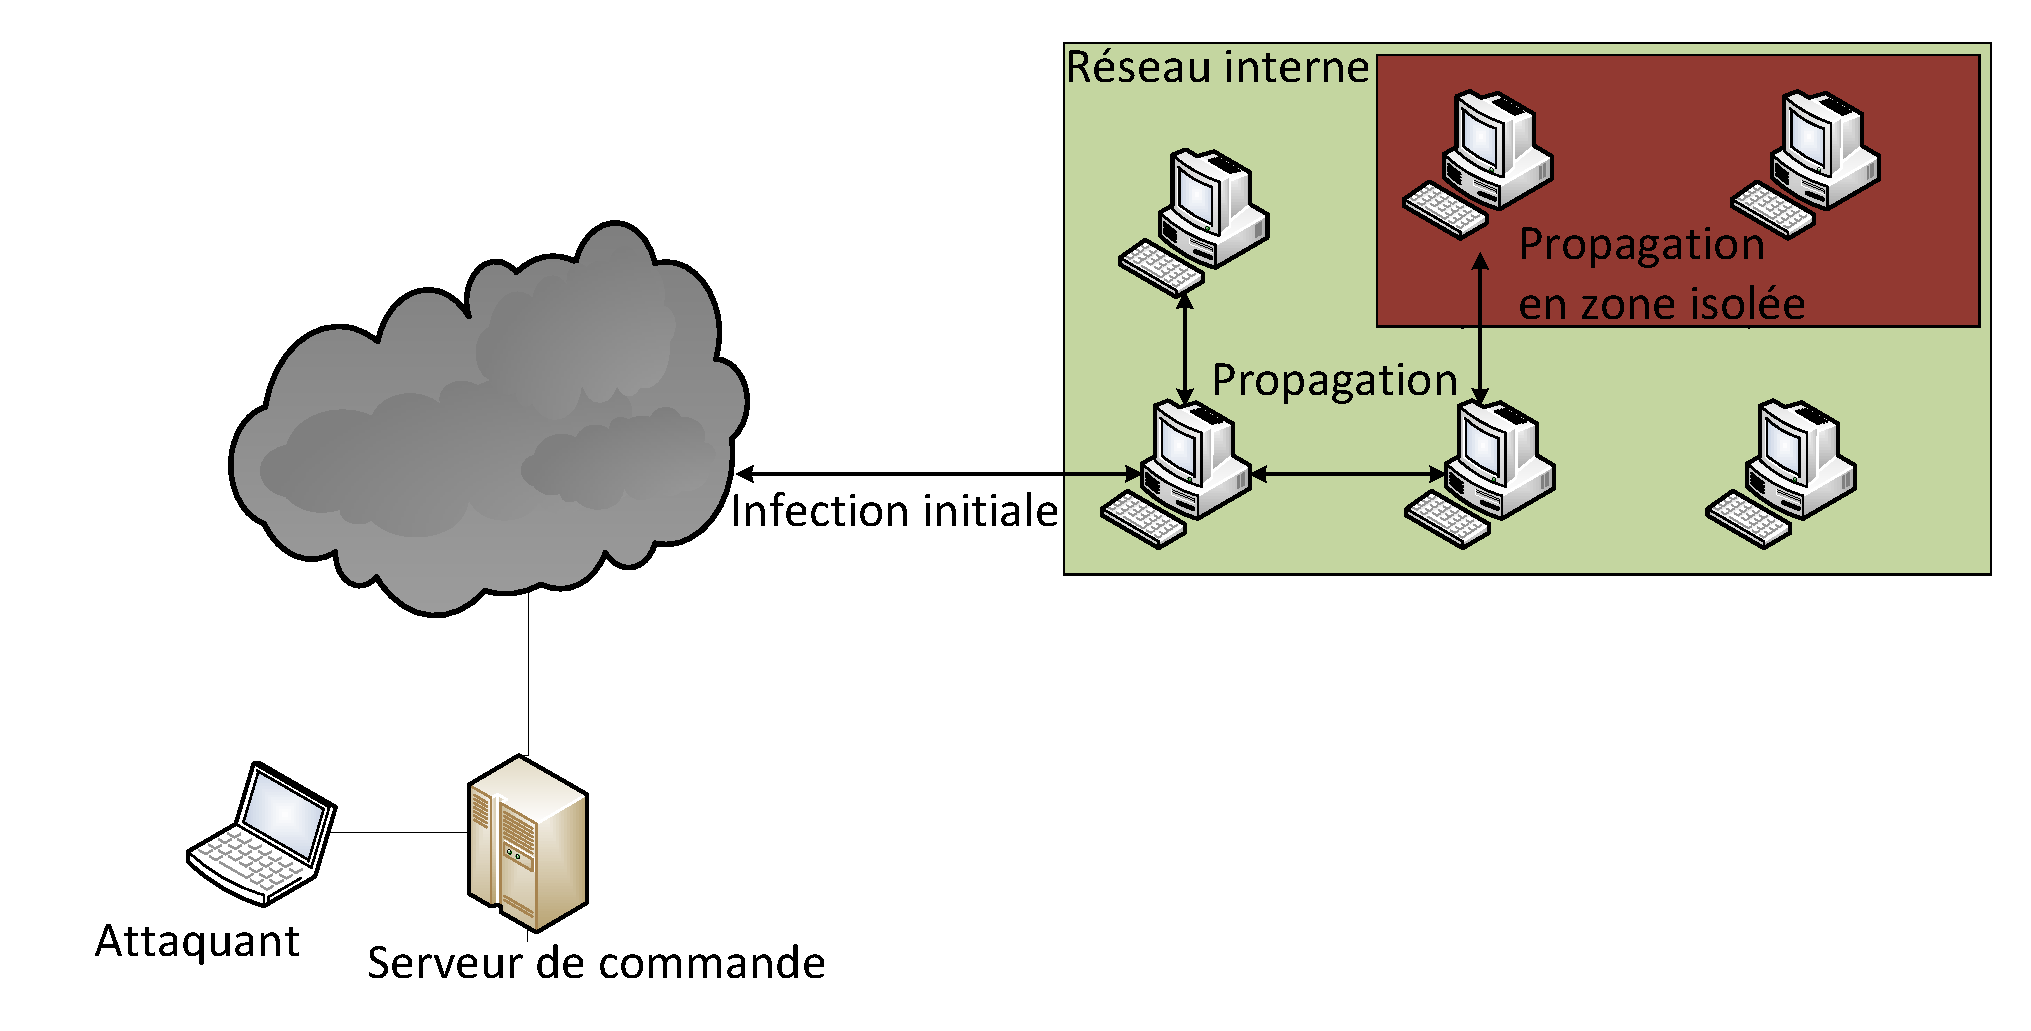
\includegraphics[width=0.5\textwidth]{img/propagationDuqu.pdf}
%  % graph11.eps: 0x0 pixel, 300dpi, 0.00x0.00 cm, bb=0 0 384 336
% \end{center}
% \caption{\Duqu's in-depth propagation technique}
% \label{fig:AThierry_propagationDuqu}
% \end{figure}


\section{Rebuilding the driver's source code}

We knew \Duqu\ shared code with \Stuxnet\ since we showed equivalent parts in the drivers' main DLLs \cite{AThierry_REAT12} and Symantec revealed similarities in the injection technique and some resources. The decompilation of \Stuxnet's driver had already be done by Amr Thabet \cite{AThierry_ThabetDriver} but we decided to decompile \Duqu's driver into C code to expose how it operates and the difference between the drivers of \Duqu\ and \Stuxnet. And actually we found singular techniques for injection and anti-detection mechanisms.
% We found singular techniques for injection and avoiding detection.

% Thus we proceeded with reversing the driver and documenting its functionalities. Our goal is to obtain a readable source code whose compiled version is close to the original binary.

% Nous savions que \Duqu\ partage du code avec Stuxnet puisque nous avons exhibé des parties équivalentes dans les DLL principales de chacun des malware \cite{AThierry_REAT12} et Symantec a détaillé des similarités dans la technique d'injection de la DLL et dans certaines ressources (exports et routines).
% Pourquoi alors s'intéresser au driver de \Duqu\ alors que celui de \Stuxnet, similaire, a été décompilé par Amr Thabet \cite{AThierry_ThabetDriver} ?
% En réalité le diable est dans les détails car l'analyse détaillée d'une souche du driver découverte en octobre 2011 en Europe (\driver) a montré de nombreuses singularités par rapport à \Stuxnet\ dans sa méthode d'injection et ses mécanismes de furtivité.

% Nous avons donc travaillé sur la rétroingénierie de cette version spécifique du driver afin d'en documenter les fonctionnalités.
% Notre objectif est d'obtenir un code compréhensible, qui compile, et dont la version compilée soit au plus proche du driver original.


\subsection{IDA's decompiler}
We used IDA's plugin "Hex-Rays Decompiler" \cite{AThierry_IDADecompiler}. It generates C pseudocode from a binary being analyzed in IDA and authorizes modifications of the C code from within the plugin's GUI. 
Unfortunately the code generated by IDA was, in our case, not directly usable: an example of the first lines of a function decompiled by IDA is given on Figure \ref{fig:AThierry_ParsePEInitial}.
Firstly the code cannot be re-compiled because some variable types, function arguments and calling conventions were not recognized by the decompiler.
Secondly the generated code is hardly readable, partly because some structures and librairies were not identified. Let us detail how to circumvent these issues.

% Nous avons utilisé le module de décompilation "Hex-Rays Decompiler", intégré à IDA sous la forme d'un plugin \cite{AThierry_IDADecompiler}. Il permet de générer un pseudo-code C à partir du fichier binaire en cours d'analyse. Il produit non seulement du code source mais facilite également sa réécriture directement à l'intérieur de l'interface graphique du plugin. % (menu {\em Open subviews Pseudocode F5}).
% Malheureusement le code en sortie n'est, dans notre cas, pas exploitable directement. D'une part le code n'est pas compilable parce que des types de variables n'ont pas été correctement reconnus et certaines conventions d'appel ne sont pas standard (non reconnues par le décompilateur). De plus le code généré est difficilement lisible, en partie parce que certaines structures n'ont pas été identifiées. Nous détaillerons dans les paragraphes suivants ces difficultés et des moyens de résolution.

In order to rebuild a consistent source code we followed an incremental protocol based on the decompiler's output. We began with commenting the whole decompiled code except for the entrypoint of the driver. We fixed compilation errors and identified missing structures. Once the entrypoint was readable and could be compiled, we added some more code that was previously commented, fixed it, and so on.

% We followed an incremental protocol in order to rebuild the source code, checking at each step that the code can be compiled and that, compiled, it is close to \Duqu's original binary.
% It consisted in :
% % Nous avons procédé de manière incrémentale afin de reconstruire le code petit à petit en vérifiant à chaque étape que le code compile et qu'une fois compilé il est équivalent à celui du binaire \driver\ original. 
% % Cela a consisté à :
% \begin{itemize}
%  \item Comment the whole code except for the entrypoint of the driver (\emph{DriverEntry}) and some global variables
%  \item Fix errors, one after the other
%  \item Compare the compiled code to the original binary, modify the code to be closer
%  \item Add more code that was previously commented and loop back to the error fixing step.
% \end{itemize}
% \begin{itemize}
%  \item Commenter tout le pseudo-code sauf la fonction du point d'entrée du driver (\emph{DriverEntry}) et les variables globales s'y rapportant
%  \item Régler chaque erreur une par une
%  \item Comparer le code compilé au binaire original, modifier le code pour s'en rapprocher
%  \item Ajouter du code auparavant commenté et revenir à l'étape de correction d'erreurs.
% \end{itemize}

% \begin{figure*}
% \begin{changemargin}{-0cm}{-0cm}
% \includegraphics[width=1.0\textwidth]{img/decompil.pdf}
% \end{changemargin}
% \caption{À gauche, le code source initialement généré par IDA. À droite, une fois le type de la variable \texttt{BaseAddress} re-défini.}
% \label{fig:AThierry_decompil}
% \end{figure*}

\subsection{Structures and types identification}

Figure \ref{fig:AThierry_ParsePEInitial} depicts the first lines of the decompiler's output for one of the driver's function.
A lot of information is missing, for instance most types are described as \texttt{int} so the kind of processing done is unknown.
We will give more details on this example to illustrate what has been done to fix the code generated by the decompiler.
Some of the constants are going to be of great help: for instance we can combine both of them 0xF750F284~XOR~0xF750B7D4~=~0x00004550 =~'PE$\backslash$0$\backslash$0', the text searched is 'PE$\backslash$0$\backslash$0' which is obfuscated with a XOR operation.

At this point we have strong suspicion that this function is used to parse PE files.
A quick dive in Microsoft's Visual C++ documentation reveals the structure PIMAGE\_NT\_HEADERS which first field is \emph{Signature}, whose value is 'PE$\backslash$0$\backslash$0' for Windows binaries. Thus the variable \texttt{v4}, which is tested against 'PE$\backslash$0$\backslash$0', might be of type PIMAGE\_NT\_HEADERS.
So we force this structure and others into IDA's decompiler in place of default \texttt{int} type, IDA then finds fields based on their offsets and updates them in the code. In some cases the structure is specific to the analyzed binary (user defined), it is possible to define them manually in the decompiler plugin.

The beginning of the fixed code is presented on Figure \ref{fig:AThierry_ParsePEFinal}, it is readable by a C developer: one sees that the function checks whether a file is a PE binary. The following part of the code will parse it and fill a user defined structure with some information (entrypoint, sections...). Besides the compiled binary of this version is very similar to the original binary. Doing this kind of analysis on the whole driver lead us to build an understandable and consistent version of the driver's source code.



% Comme on peut s'en rendre compte sur la partie gauche de la figure \ref{fig:AThierry_decompil}, le décompilateur n'arrive pas toujours à déterminer le type d'une variable.
% On prend l'exemple de la fonction \texttt{ParsePE}, utilisée pour chercher des informations dans les binaires chargés en mémoire.
% On part donc à la pêche aux indices : ici le test sur la valeur magique "\texttt{MZ}" nous laisse à penser que la fonction porte sur un traitement de l'entête d'un fichier exécutable au format PE, ce qui nous permet d'en déduire que la variable \texttt{BaseAddress} est un pointeur sur une structure \texttt{IMAGE\_DOS\_HEADER}. Une fois le type de la variable correctement défini, IDA identifie automatiquement le nom du champ de la structure à l'{\em offset} indiqué nous épargnant de longues recherches dans la documentation de Microsoft (par exemple l'{\em offset} 60 soit 0x3C en hexadécimal correspond au champ \texttt{e\_lFanew} de la structure \texttt{IMAGE\_DOS\_HEADER}). Si la structure est propre au programme analysé, nous pouvons la définir à travers le plugin de décompilation après une analyse manuelle.

% \begin{figure}
% %\begin{changemargin}{-2cm}{-2cm}
% \includegraphics[width=1.0\textwidth]{AThierry/img/pseudocode-final.pdf}
% %\end{changemargin}
% \caption{Modification du code source depuis le plugin d'IDA}
% \label{fig:pseudocodefinal}
% \end{figure}

% Au final, nous avons retouché le code pour obtenir un code compréhensible pour un développeur C (figure \ref{fig:AThierry_ParsePEFunction}).
% Ce n'est pas encore un code ``propre'' : par exemple un développeur n'aurait pas utilisé de \emph{goto} pour gérer un traitement commun à la fin d'une condition mais l'aurait plutôt placé après la disjonction des cas, et il aurait rajouté une clause \emph{else} pour le cas par défaut. Après cette réorganisation, les objectifs sont atteints : pour la fonction \texttt{ParsePE}, le code (re)compilé est proche du binaire original, et le code source reconstruit est exploitable.
% 
% La lisibilité du code ainsi obtenu nous permet de détecter une erreur de programmation comme à la deuxième ligne ici :
% 
%  \begin{center}
%  \begin{changemargin}{-1cm}{-1cm}
% \begin{lstlisting}[language={C}]
%   else if ((pFileHeader->Machine ^ 0xDE67) == (IMAGE_PE_x86_MACHINE ^ 0xDE67) 
%            && (pOptionHeader->Magic ^ 0x5A08) == IMAGE_PE32_PLUS_MAGIC 
%            && pFileHeader->SizeOfOptionalHeader == 0xF0 ) // 0x5803 64bits
% \end{lstlisting}
% \hspace{1cm} Au lieu de :
% \begin{lstlisting}[language={C}]
%   else if ((pFileHeader->Machine ^ 0xDE67) == (IMAGE_PE_x86_MACHINE ^ 0xDE67) 
%            && (pOptionHeader->Magic ^ 0x5A08) == (IMAGE_PE32_PLUS_MAGIC ^ 0x5A08) 
%            && pFileHeader->SizeOfOptionalHeader == 0xF0 ) // 0x5803 64bits
% \end{lstlisting}
%  \end{changemargin}
%  \end{center}
% 
% Le test mis en place omet un XOR sur la constante IMAGE\_PE32\_PLUS\_MAGIC. Ce test devrait permettre de reconnaître un binaire 64 bits et de définir une table d'import en conséquence. Avec cette erreur, \Duqu\ est incapable de parser un binaire 64 bits (un code d'erreur est renvoyé). De fait cette version du driver ne fonctionne pas sur un Windows 64 bits.

\begin{figure}
% \scriptsize

\begin{small}\begin{lstlisting}[language={C}]
signed int __cdecl sub_12F36(int a1,
		     int a2, int a3)
{
  int v4; // eax@3
  unsigned __int16 v5; // cx@4
  int v6; // ecx@7

  v4 = a2 + *(_DWORD *)(a2 + 60);
  if (*(_DWORD *)v4 ^ 0xF750F284
	           != 0xF750B7D4)
    return 1;
\end{lstlisting}\end{small}
\caption{First 10 lines of the ParsePE function as decompiled by IDA\label{fig:AThierry_ParsePEInitial}}
\end{figure}

\begin{figure}
% \scriptsize
\begin{small}\begin{lstlisting}[language={C}]
NTSTATUS __cdecl ParsePE(
 __out PEDataPtr pPEData, 
 __in PIMAGE_DOS_HEADER BaseAddress,
 __in int flag){
PVOID infosPE;
PIMAGE_DOS_HEADER pDosHeader;
PIMAGE_NT_HEADERS pNtHeader;

pNtHeader = (DWORD)infosPE +
		  infosPE->e_lfanew;
if ((pNtHeader->Signature ^ 0xF750F284)
  != (IMAGE_NT_SIGNATURE ^ 0xF750F284)) 
    return STATUS_WAIT_1; 
\end{lstlisting}\end{small}
\caption{First 10 lines of the fixed ParsePE function\label{fig:AThierry_ParsePEFinal}}
\end{figure}
% 
% \begin{figure*}
% \scriptsize
% \begin{lstlisting}[language={C}]
% NTSTATUS __cdecl ParsePE(
%       __out PEDataPtr pPEData, 
%       __in PIMAGE_DOS_HEADER BaseAddress,
%       __in int flag)
% {
%   PVOID infosPE; //IMAGE_NT_HEADER; 
%   PIMAGE_DOS_HEADER  pDosHeader     = NULL;
%   PIMAGE_NT_HEADERS  pNtHeader      = NULL;
%   PIMAGE_FILE_HEADER  pFileHeader   = NULL;
%   PIMAGE_OPTIONAL_HEADER32  pOptionHeader = NULL;
%   PVOID pExportTableRVA; 
% 
%   infosPE=(PIMAGE_DOS_HEADER)BaseAddress; 
%   if (((PIMAGE_DOS_HEADER)infosPE)->e_magic != 'ZM' )
%     return STATUS_WAIT_1;
% 
%   pNtHeader = (PIMAGE_NT_HEADERS32)((DWORD)infosPE + ((PIMAGE_DOS_HEADER)infosPE)->e_lfanew);
%   // hash of 'P' 'E' '0' '0' (0x00004550) => 0x0F750B7D4
%   if ( (pNtHeader->Signature ^ 0xF750F284) != (IMAGE_NT_SIGNATURE ^ 0xF750F284)) 
%     return STATUS_WAIT_1; 
% 
%   pFileHeader = (PIMAGE_FILE_HEADER)&pNtHeader->FileHeader;
%   pOptionHeader = (PIMAGE_OPTIONAL_HEADER32)&((PIMAGE_NT_HEADERS32)infosPE)->OptionalHeader;
%   if ((pFileHeader->Machine ^ 0x594F) == (IMAGE_PE_i386_MACHINE ^ 0x594F)) 
%   {
%     if ((pOptionHeader->Magic ^ 0x5908) == (IMAGE_PE32_MAGIC ^ 0x5908) && (pFileHeader->SizeOfOptionalHeader == 0xE0 ))  
%     {
%       pPEData->Status = 0;
%       pExportTableRVA = (PVOID)&(pOptionHeader->DataDirectory[IMAGE_DIRECTORY_ENTRY_EXPORT]).VirtualAddress;  
% 
% Continue:
%       pPEData->ExportTableRVA=pExportTableRVA;     
%       pPEData->dwSizeOfImage = pOptionHeader->SizeOfImage;  
%       pPEData->lpDataDir=pFileHeader->SizeOfOptionalHeader + (BYTE *)&(pFileHeader->Characteristics) + sizeof(WORD);                                                              
%       pPEData->ResourceDataDir=(ULONG)infosPE;                        
%       pPEData->PEAddress1=pPEData->PEAddress2;                        
%       pPEData->wNumberOfSections=pFileHeader->NumberOfSections;       
%       pPEData->PEAddress2=(PIMAGE_DOS_HEADER)&((PIMAGE_NT_HEADERS32)infosPE)->Signature; 
%       return STATUS_SUCCESS;
%      }
%   }
%   else if ((pFileHeader->Machine ^ 0xDE67) == (IMAGE_PE_x86_MACHINE ^ 0xDE67) 
%            && (pOptionHeader->Magic ^ 0x5A08) == IMAGE_PE32_PLUS_MAGIC 
%            && pFileHeader->SizeOfOptionalHeader == 0xF0 ) // 0x5803 64bits
%   {
%     pPEData->Status = 1;
%     pExportTableRVA = (PVOID)&(pOptionHeader->DataDirectory[IMAGE_DIRECTORY_ENTRY_RESOURCE]).VirtualAddress; 
%     goto Continue;
%   }
%   return STATUS_WAIT_1;
% }
% \end{lstlisting}
% \caption{Code source final de la fonction ParsePE\label{fig:AThierry_ParsePEFunction}}
% \end{figure*}

% \clearpage
% \subsection{Conventions d'appel}
% 
% Pour chaque routine, IDA cherche à déterminer la convention d'appel utilisée à partir des registres qui sont lus avant d'être écrits (paramêtres) et ceux écrits sans être lus après (valeur de retour). Si ces registres correspondent à un appel classique, il l'annote dans le code C pour que le compilateur respecte la convention. Les conventions d'appel de Microsoft Visual C++ sont données Figure \ref{fig:AThierry_callingconvention}, l'appel par défaut étant \emph{thiscall}. Dans le cas où il ne détermine pas la convention, il annote les registres d'entrée et de sortie en notant qu'il s'agit d'un appel non conventionnel (\emph{usercall}) et met la définition de la fonction en commentaire (ici les arguments sont passés dans les registres \texttt{edi} et \texttt{esi}) :
% \begin{changemargin}{-0.4cm}{-0.4cm}
% \begin{lstlisting}[language={C}, escapechar=!]
% !//! int __usercall SearchForCodeInSystem<eax>(int *a1<edi>, int a2<esi>);
% \end{lstlisting}
% \end{changemargin}
% 
% Une convention d'appel non standard est détectée dans le cas où une partie de la fonction a été écrite directement en assembleur ou à la suite d'une optimisation faite par le compilateur. On doit alors réécrire la fonction à la main (en partie en assembleur) ou choisir à la main une convention d'appel.
% 
% \begin{figure}
% \begin{center}
% \begin{tabular}{|l|c|c|c|c|}
% \hline 
% Convention & Arguments & \emph{this} (C++) & Retour & Nettoie la pile\\
% \hline
% C (\_\_cdelcl) & pile & (argument) & eax & appelant\\
% Standard (\_\_stdcall) & pile & (argument) & eax & appelé\\
% Thiscall (\_\_thiscall) & pile & ecx & eax & appelé\\
% Fastcall (\_\_fastcall) & ecx, edx, pile & (argument) & eax & appelé\\
% \hline
% \end{tabular}
% \end{center}
% \caption{Conventions d'appel dans leur version Visual C++}
% \label{fig:AThierry_callingconvention}
% \end{figure}

\section{Functional analysis from the source code}

Now that the source code has been rebuilt, let us detail how it operates.
There are two main phases, the first one consists in setting up the driver: it asks the operating system for notifications when a binary is loaded, and initializes stealth mechanisms.
The second one is triggered when it receives notifications: the driver infects the target binary by injecting \Duqu's DLL into \service, then activates the payload.

% Une fois le code du driver reconstitué, décrivons en détail son fonctionnement.
% Il y a deux phases principales, la première consiste en la mise en place du driver : il demande au système d'être notifié en cas de chargement de binaires et initialise ses mécanismes de furtivité.
% La seconde phase est lancée lorsque des notifications sont signalées chargeant un binaire cible. Le driver infecte alors le binaire en y injectant la DLL de \Duqu\ puis celle-ci active la charge finale.

\subsection{Initialisation of the driver during boot}
Recall that on Windows, the startup order of drivers is determined by their \texttt{Group} key in the registry. \Duqu's \driver, belonging to the "network" group, is activated before the hardware abstraction layer (HAL) is loaded into memory.

% La séquence de démarrage des drivers système sous Windows est déterminée par le positionnement de la clé de registre \texttt{Group}. Ainsi en fonction de son groupe d'appartenance (\driver\ fait partie du groupe "network"), le driver sera démarré plus ou moins tôt lors de la séquence de boot. Le système d'exploitation donne automatiquement la main aux drivers prioritaires avant même que la couche d'abstraction matérielle (HAL) ne soit chargée en mémoire. 

Once started, \driver\ allocates 512 bytes for storing a pointer array of functions shared by various callback routines. Then it decrypts some internal parameters, revealing the name and path of the registry key used for configuring the injection.
% along with the name the driver registers for itself within the operating system.

% Le driver, une fois démarré, commence par allouer un emplacement mémoire de 512 octets destiné à contenir un tableau de pointeurs de fonctions partagées entre les différentes routines de "callback". A la suite de cela, il passe au déchiffrement de ses paramètres internes (avec la fonction donnée en figure \ref{fig:AThierry_decrypt}) nous révélant ainsi le nom et l'emplacement de la clé de registre utilisée pour la configuration de "l'injection" mais également le nom sous lequel le driver va s'enregistrer au près du gestionnaire.  
% \begin{figure*}
% \scriptsize
% \begin{lstlisting}[language={C}]
%  void __fastcall decode_parameters(
%       __in PUNICODE_STRING RegistryPath)
% {
%   ULONG dwSeed; 
%   UINT32 dwCount; 
% 
%   dwSeed = 0x7EF640F0;
%   dwCount = 0;
%   
%   do
%   {
%     g_DefaultParamCrypted[dwCount++] ^= (char) dwSeed;
%     dwSeed = ((((dwSeed & 0xFFFFFFFB) << 28) | (dwSeed >> 5)) * (((dwSeed & 0xFFFFFFFB) << 28) 
%     | (dwSeed >> 5)) / 0x8677 + 0x787C956A * (((dwSeed & 0xFFFFFFFB) << 28) | (dwSeed >> 5)) + 1) 
%     ^ (((dwSeed & 0xFFFFFFFB) << 28) | (dwSeed >> 5));
%   } while (dwCount < 428 );
% 
%   if ( (char)g_LocalParameters == 0) { 
%       //Recopie le chemin de la cle de registre lorsque cela est necessaire
%       memcpy((void *)&g_LocalParameters, RegistryPath->Buffer, RegistryPath->Length);
%   }
% }
% \end{lstlisting}
% \caption{Routine de déchiffrement utilisée pour les paramètres internes (également utilisée sur la DLL à injecter).}
% \label{fig:AThierry_decrypt}
% \end{figure*}


If the decryption succeeded, the driver checks its execution mode. If it is in debug or fail-safe mode, the driver halts, otherwise it creates a device named \texttt{\{624409B3-4CEF-41c0-8B81-7634279A41E5\}} and defines a list of control commands that the device can process.
% Si le déchiffrement s'est correctement déroulé, vient alors la vérification du mode d'exécution : soit le système s'avère être en mode sans échec ou en mode débogage, dans ce cas le driver termine son exécution ; soit en mode normal alors il commence par créer un device répondant au doux nom de $\backslash$\texttt{Device}$\backslash$\texttt{\{624409B3-4CEF-41c0-8B81-7634279A41E5\}} puis il définit la liste des commandes de contrôle qu'il sera à même de traiter (une grande majorité des commandes commencent par  \texttt{IRP\_MJ\_} tels que \texttt{IRP\_MJ\_CREATE}, \texttt{IRP\_MJ\_READ}, etc.).

That being done, it registers two callback functions within the kernel's event handler. The first is required by the operating system: it is used to create an access point  ($\backslash$\texttt{Device}$\backslash$\texttt{Gpd0}) and a link ($\backslash$\texttt{DosDevices}$\backslash$\texttt{GpdDev}) to the driver, and attaches the device to a memory stack.
The second function will be called when the driver is initialized or reinitialized, it is inserted in a waiting list of events.
% Ceci étant fait, il enregistre auprès du gestionnaire d'événements interne du noyau, deux fonctions de rappel ({\em callback function}). La première est nécessaire au gestionnaire du \texttt{Plug and Play} (\texttt{PnP}). On y trouve des opérations classiques pour un driver, à savoir la création d'un point d'accès sur celui-ci ($\backslash$\texttt{Device}$\backslash$\texttt{Gpd0}), ainsi qu'un lien ($\backslash$\texttt{DosDevices}$\backslash$\texttt{GpdDev}) et enfin l'attachement de l'objet \texttt{Device} à une pile mémoire. Quant à la seconde, elle sera exécutée lorsque le driver devra être initialisé ou réinitialisé (à la différence de la première, cette fonction est insérée dans une liste d'attente d'événements et supprimée à l'issue de son traitement). 

This second function waits until the Windows kernel is totally loaded: it checks if the DLL \texttt{hal.dll} is loaded, if not, the function is once again inserted into the events waiting list (for at most 200 times).
% Cette seconde fonction embarque un mécanisme d'attente de fin de chargement du noyau Windows. Pour cela, une fonction vérifie qu'il est possible d'accéder à la DLL \texttt{hal.dll}. Si tel n'est pas le cas, la fonction de réinitialisation est de nouveau insérée dans la file d'attente des traitements pour un maximum de 200 fois. 
When the system is ready, an access point $\backslash$\texttt{Device}$\backslash$\texttt{Gpd1} is created and linked to a request processing function. 
At that point librairies are available for \Duqu's injection.
% At that point the driver is able to communicate with a user mode (ring 3) application.
% Lors de la fin de chargement du système, un point d'accès $\backslash$\texttt{Device}$\backslash$\texttt{Gpd1} est alors créé puis une routine de traitement des requêtes lui est associé. À ce stade le driver est à même de dialoguer avec une application s'exécutant en mode utilisateur (ring 3). 

\subsubsection{Stealth techniques}
The driver acts like a rootkit because it avoids directly using suspicious system calls. Indeed those system calls might be monitored by an antivirus. Typically the function \texttt{ZwAllocateVirtualMemory} can be used to allocate memory space into any process, for instance to inject code into any target process. Besides, in order to hook the entrypoint of a system binary, \Duqu\ also needs the function \texttt{ZwProtectVirtualMemory} that is deliberately not exported by the kernel. This function modifies the permissions of a memory block and can be used to make a code section writable or execute code in a data section. \Duqu\ was built to find \texttt{ZwProtectVirtualMemory}'s memory address without using imports.

% The driver is looking for the memory locations of \texttt{ZwAllocateVirtualMemory} and \texttt{ZwProtectVirtualMemory} while avoiding detection.
The two functions are implemented in the Windows kernel (in \texttt{Ntoskrnl.exe} or \texttt{ntkrnlpa.exe}, depending on the version).
The driver inspects every module (DLLs and EXE files) loaded by the OS during boot until it finds one of the two target kernel files.

% A first function is in charge of scanning every module (DLLs and executable files) loaded by the OS during boot until it finds one of the two target kernel files. The list of loaded modules is obtained through the kernel function \texttt{ZwQuerySystemInformation}.
Once the file is found, the driver uses the function \texttt{ParsePE} to examine it closely.
It searches, in that kernel file, a call to \texttt{ZwAllocateVirtualMemory} (whose address is known from the export table) followed by the opcode \texttt{push~104h} and another (near) call to an unknown function. If this pattern, shown in Figure \ref{fig:AThierry_CallZwProtect}, is found, the target address of this last call is considered to be \texttt{ZwProtectVirtualMemory}.
At this point the memory addresses of both functions are known.
% The kernel file is a \texttt{PE} binary, the function checks it for magic values such as '\texttt{MZ}', '\texttt{IMAGE\_NT\_SIGNATURE}', '\texttt{IMAGE\_PE\_i386\_MACHINE}, '\texttt{IMAGE\_PE\_x86\_MACHINE}', '\texttt{IMAGE\_PE32\_MAGIC}' or '\texttt{IMAGE\_PE32\_PLUS\_MAGIC}', then it locates the entrypoint, the sections and the export table.
% The function is specifically interested in the section containing executable code (\texttt{.text} or \texttt{PAGE}).%, with access rights set as \texttt{IMAGE\_SCN\_MEM\_EXECUTE}, \texttt{IMAGE\_SCN\_MEM\_READ} and \texttt{IMAGE\_SCN\_CNT\_CODE}).


\begin{figure*}
\scriptsize
\begin{lstlisting}[language={[x86masm]Assembler}, escapechar=~]
(01) PAGE:004ED1AD                  loc_4ED1AD: [...]                      
(02) PAGE:004ED1BC 50               push    eax             ; BaseAddress
(03) PAGE:004ED1BD 57               push    edi             ; ProcessHandle
(04) PAGE:004ED1BE E8 19 8C F1 FF   ~\textcolor{red}{\texttt{call    DS:ZwAllocateVirtualMemory}}~
(05) PAGE:004ED1C3 3B C3            cmp     eax, ebx
(06) PAGE:004ED1C5 8B 4D FC         mov     ecx, [ebp+BaseAddress]
(07) PAGE:004ED1C8 89 4E 0C         mov     [esi+0Ch], ecx
(08) PAGE:004ED1CB 7C 2E            jl      short loc_4ED1FB
(09) PAGE:004ED1CD 38 5D 0B         cmp     byte ptr [ebp+ProcessHandle+3], bl
(10) PAGE:004ED1D0 74 27            jz      short loc_4ED1F9
(11) PAGE:004ED1D2 8B 45 D0         mov     eax, [ebp+var_30]
(12) PAGE:004ED1D5 89 45 F8         mov     [ebp+ProtectSize], eax
(13) PAGE:004ED1D8 8D 45 F4         lea     eax, [ebp+OldProtect]
(14) PAGE:004ED1DB 50               push    eax             ; OldProtect
(15) PAGE:004ED1DC 68 04 01 00 00   ~\textcolor{red}{\texttt{push    104h}}~
(16) PAGE:004ED1E1 8D 45 F8         lea     eax, [ebp+ProtectSize]
(17) PAGE:004ED1E4 50               push    eax             ; ProtectSize
(18) PAGE:004ED1E5 8D 45 FC         lea     eax, [ebp+BaseAddress]
(19) PAGE:004ED1E8 50               push    eax             ; BaseAddress
(20) PAGE:004ED1E9 57               push    edi             ; ProcessHandle
(21) PAGE:004ED1EA E8 93 96 F1 FF   ~\textcolor{red}{\texttt{call    loc\_406882}}~ ; ZwProtectVirtualMemory
(22) PAGE:004ED1EF 3B C3            cmp     eax, ebx
\end{lstlisting}
% \end{framed}
\caption{Function calling ZwProtectVirtualMemory.\label{fig:AThierry_CallZwProtect}}
\end{figure*}

% La fonction recherchée contient l'opcode \texttt{push 104h} (encodé en \texttt{68 04 01 00 00}) et réalise un \texttt{call} (encodé en \texttt{E8}) un peu plus loin dans le code.
% Sachant que cette fonction effectue au préalable un appel vers la fonction \texttt{ZwAllocateVirtualMemory}, la recherche remonte jusqu'à trouver cet appel (l'adresse du \texttt{call} est comparée à celle de la fonction \texttt{ZwAllocateVirtualMemory} exportée par le noyau), puis redescend au prochain \texttt{call} (à l'adresse \texttt{0x004ED1EA}) qui est l'appel vers \texttt{ZwProtectVirtualMemory} recherché.
\paragraph{Avoiding hooks.}
It is firstly checked that the two functions are located inside the kernel's memory addresses and not in user space which would indicate an obvious hook to a monitored function.
Secondly an integrity mask applying a logical \texttt{AND} is applied on the first 32 bytes of both functions. The mask is the same for the two functions and is shown on Figure \ref{fig:AThierry_matching}.
If the functions pass both tests, their addresses are considered valid and are kept for a future stealthy use.

% Le processus vérifie dans un premier temps que l'adresse trouvée pour la fonction \texttt{ZwProtectVirtualMemory} est bien située dans une fonction du noyau pour s'assurer qu'elle n'est pas déroutée vers une fonction de surveillance.
% Dans un second temps, elle contrôle son intégrité par l'application d'un masque sur les 32 octets composant la routine avec un \texttt{AND} logique (voir figure \ref{fig:AThierry_matching}). Ces vérifications sont également effectuées pour la fonction \texttt{ZwAllocateVirtualMemory}.

% \begin{figure}
% \scriptsize
% % \begin{framed}
% \begin{changemargin}{-1cm}{-1cm}
% \begin{lstlisting}[language={[x86masm]Assembler}]
% .text:0044A0EE                 add     esi, eax
% .text:0044A0F0                 mov     [ebp+BaseAddress], esi
% .text:0044A0F3                 push    4               ; Protect
% .text:0044A0F5                 push    eax             ; AllocationType
% .text:0044A0F6                 lea     eax, [ebp+AllocationSize]
% .text:0044A0F9                 push    eax             ; AllocationSize
% .text:0044A0FA                 push    ebx             ; ZeroBits
% .text:0044A0FB                 lea     eax, [ebp+BaseAddress]
% .text:0044A0FE                 push    eax             ; BaseAddress
% .text:0044A0FF                 push    0FFFFFFFFh      ; ProcessHandle
% .text:0044A101                 call    ZwAllocateVirtualMemory
% .text:0044A106                 mov     [ebp+var_28], eax
% .text:0044A109                 cmp     eax, ebx
% .text:0044A10B                 jl      short loc_44A140
% .text:0044A10D                 mov     eax, [ebp+BaseAddress]
% .text:0044A110                 mov     [edi], eax
% .text:0044A112                 jmp     short loc_44A140
% .text:0044A114 ; -----------------------------------------------------------
% .text:0044A114
% .text:0044A114 loc_44A114:                             
% .text:0044A114                 add     ecx, 1000h
% .text:0044A11A                 mov     [edi], ecx
% .text:0044A11C                 push    104h            ; Protect
% .text:0044A121                 push    eax             ; AllocationType
% .text:0044A122                 lea     eax, [ebp+AllocationSize]
% .text:0044A125                 push    eax             ; AllocationSize
% .text:0044A126                 push    ebx             ; ZeroBits
% .text:0044A127                 lea     eax, [ebp+BaseAddress]
% .text:0044A12A                 push    eax             ; BaseAddress
% .text:0044A12B                 push    0FFFFFFFFh      ; ProcessHandle
% .text:0044A12D                 call    ZwAllocateVirtualMemory
% .text:0044A132                 mov     [ebp+var_28], eax
% \end{lstlisting}
% \end{changemargin}
% % \end{framed}
% \caption{Fonction faisant appel à ZwAllocateVirtualMemory.\label{fig:CallZwAlloc}}
% \end{figure}


\begin{figure}
\begin{center}
 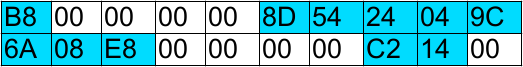
\includegraphics[width=0.48\textwidth]{presentation/masque/octetsmasque.png}
 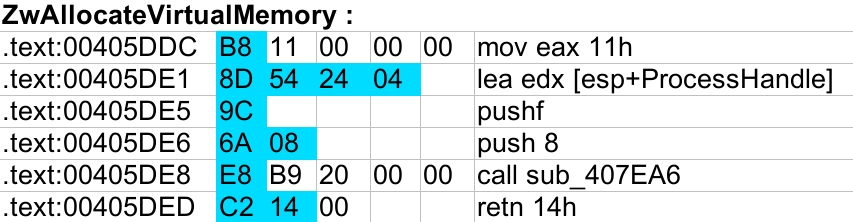
\includegraphics[width=0.48\textwidth]{presentation/masque/masqueZwAllocate.png}
 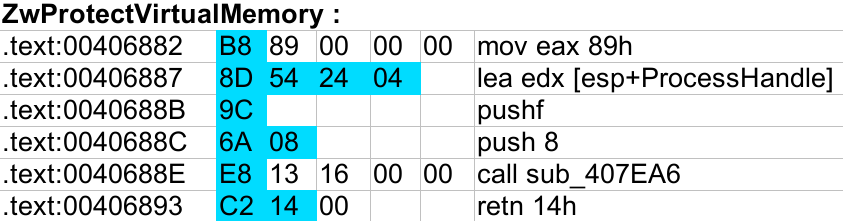
\includegraphics[width=0.48\textwidth]{presentation/masque/masqueZwProtect.png}
\end{center}
\caption{Integrity mask applied on ZwAllocateVirtualMemory and \mbox{ZwProtectVirtualMemory}. Values filled in gray are those checked.}
\label{fig:AThierry_matching}
\end{figure}

% Lorsque le driver est exécuté sur un système Windows 2000, la technique employée diffère. Cette fois-ci une fonction va parcourir le code à la recherche non pas de l'opcode \texttt{push 104h} mais de \texttt{mov eax, 77h} (encodé en \texttt{B8 77 00 00 00}) afin de localiser directement la routine \texttt{ZwProtectVirtualMemory} (voir la figure \ref{fig:ZwProtectVirtualMemory}) puis de vérifier que chaque opcode est semblable à celui contenu dans le code du driver. 

% \begin{figure}
% % \begin{framed}
% \scriptsize
% \begin{changemargin}{-1cm}{-1cm}
% \begin{lstlisting}[language={[x86masm]Assembler}]
% .text:00400F2A B8 77 00 00 00  mov   eax, 77h
% .text:00400F2F 8D 54 24 04     lea   edx, [esp+ProcessHandle]
% .text:00400F33 CD 2E           int   2Eh    ; DOS 2+ internal - EXECUTE COMMAND
% .text:00400F33                ; DS:SI -> counted CR-terminated command string
% .text:00400F35 C2 14 00        retn  14h
% \end{lstlisting}
% \end{changemargin}
% % \end{framed}
% \caption{Appel système de la fonction \texttt{ZwProtectVirtualMemory} sous Windows 2000.\label{fig:ZwProtectVirtualMemory}}
% \end{figure}

% A présent, l'adresse de la fonction \texttt{ZwProtectVirtualMemory} peut être mémorisée pour une future utilisation discrète. 

\subsubsection{Initialization of shared memory}
A shared memory space is allocated and used as a link between the driver's  callback functions and the kernel. It is to be filled with, amongst others, infection parameters decrypted from the registry and an import table giving access to \krn\ and kernel functions. This import table will be used by both the executable code that \Duqu\ is going to inject and the payload.

% Vient alors l'initialisation d'un espace mémoire partagé servant de lien entre les différentes fonctions de rappel au sein du noyau (ring 0). Il va servir à stocker, entre autres, les paramètres d'infection extraits depuis la base de registre une fois déchiffrés, mais également une structure (voir la figure \ref{fig:AThierry_InjectedDataStruct}) donnant accès à des fonctions système situées dans la DLL Kernel32.dll. Enfin, pour ses besoins interne, il va constituer une table d'import donnant accès à des fonctions situées au c\oe ur du noyau (voir la figure \ref{fig:AThierry_NtoskrnlIAT}). Cette table d'import pourra être utilisée par la suite par les différents codes injectés ainsi que la charge finale.
% \begin{figure*}
% % \begin{framed}
% \scriptsize
% \begin{lstlisting}[language={C}]
% typedef struct _INJECTEDDATA  
% { 
% LONGLONG Kernel32Imagebase;      // Adresse de base de kernel32.dll
% LONGLONG VirtualAlloc;           // Pointeurs sur les fonctions de Kernel32 utilisees par le code injecte
% LONGLONG VirtualFree;           
% LONGLONG GetProcAddress;   
% LONGLONG GetModuleHandleA; 
% LONGLONG LoadLibraryA;      
% LONGLONG LoadLibraryW;     
% LONGLONG lstrcmpA;         
% LONGLONG lstrcmpiA;        
% LONGLONG GetVersionExA;    
% LONGLONG DeviceIoControl;  
% LONGLONG InjectedSupModuleStart;  // Pointeur sur le debut de la memoire allouee dans le processus cible
% LONGLONG InjectedSupModuleMZoffset; // Offset du debut du code tremplin injecte
% LONGLONG InjectedSupModuleSize;  // Taille du code tremplin injecte
% LONGLONG InjectedDLLImagebase;   // Pointeur sur le debut de la DLL injectee             
% ULONG EntryPoint1stDword;        // Sauvegarde des douze premiers octets du point d'entree de la cible
% ULONG EntryPoint2snDword;  
% ULONG EntryPoint3rdDword;  
% ULONG Reserved15;                   
% ULONG OldMemProtect;             // Sauvegarde des droits d'acces originaux
% ULONG Reserved17;                   
% HANDLE handle;                   // Sauvegarde de l'Handle permettant de communiquer avec le driver depuis l'espace utilisateur
% ULONG Reserved18;                
% }_INJECTEDDATA, *PINJECTEDDATA;
% \end{lstlisting}
% % \end{framed}
% \caption{Structure mémorisée dans un espace mémoire partagé.\label{fig:AThierry_InjectedDataStruct}}
% \end{figure*}
  
% \begin{figure*}
% % \begin{framed}
% \scriptsize
% %   g_RtlGetVersionADDR = 0;
% %   g_KeAreAllApcsDisabledADDR = 0;
% %   g_PsGetProcessSessionIdADDR = 0;
% %   g_PsGetProcessPebADDR = 0;
% %   g_PsSetLoadImageNotifyRoutineADDR = 0;
% %   g_ZwAllocateVirtualMemoryADDR = 0;
% %   g_KeStackAttachProcessADDR = 0;
% %   g_KeUnstackDetachProcessADDR = 0;
% \begin{lstlisting}[language={C}]
% int *__cdecl InitializeIAT()
% {
%   PIMAGE_DOS_HEADER pBaseAddress; 
%   int KeUnstackDetachProcessTmp; 
%   struct _PEData pedata;
%   PEDataPtr pPEData=NULL; 
% 
%   pBaseAddress = SearchNtoskrnl();
% 
%   if ( pBaseAddress )
%   {
%     if ( !ParsePE((PEDataPtr)&pPEData, pBaseAddress,1) )
%     {
%       // Recherche de la fonction PsSetLoadImageNotifyRoutine()
%       g_PsSetLoadImageNotifyRoutineADDR = GetApiFromKernel32((PEDataPtr)&pPEData, 0x0AA67394D); 
%       // Recherche de la fonction ZwAllocateVirtualMemory()
%       g_ZwAllocateVirtualMemoryADDR     = GetApiFromKernel32((PEDataPtr)&pPEData, 0x6DFD9339); 
%       // Recherche de la fonction KeStackAttachProcess()
%       g_KeStackAttachProcessADDR        = GetApiFromKernel32((PEDataPtr)&pPEData, 0x0A81306FD); 
%       // Recherche de la fonction KeUnstackDetachProcess()
%       KeUnstackDetachProcessTmp       = GetApiFromKernel32((PEDataPtr)&pPEData, 0x7AFE8755); 
%       g_KeUnstackDetachProcessADDR = KeUnstackDetachProcessTmp;
%       if ( g_PsSetLoadImageNotifyRoutineADDR )
%       {
%         if ( g_ZwAllocateVirtualMemoryADDR && g_KeStackAttachProcessADDR 
%               && KeUnstackDetachProcessTmp && !IsWin2kSystem() )
%         {
%           // Recherche de la fonction RtlGetVersion()
%           g_RtlGetVersionADDR         = GetApiFromKernel32((PEDataPtr)&pPEData, 0x0CA5EF8B8); 
%           // Recherche de la fonction KeAreAllApcsDisabled()
%           g_KeAreAllApcsDisabledADDR  = GetApiFromKernel32((PEDataPtr)&pPEData, 0x0B08DC9B0);
%           // Recherche de la fonction PsGetProcessSessionId()
%           g_PsGetProcessSessionIdADDR = GetApiFromKernel32((PEDataPtr)&pPEData, 0x885399FC);  
%           // Recherche de la fonction PsGetProcessPeb()
%           g_PsGetProcessPebADDR       = GetApiFromKernel32((PEDataPtr)&pPEData, 0x5A68953C); 
%         }
%       }
%     }
%   }
%   return &g_RtlGetVersionADDR;
% }
% \end{lstlisting}
% % \end{framed}
% \caption{Création de la table d'import des fonctions système issues du noyau.\label{fig:AThierry_NtoskrnlIAT}}
% % (La recherche des fonctions depuis la table d'export du fichier Ntoskrnl est réalisée en comparant le hash du nom à sa valeur calculée à l'avance).
% \end{figure*}

The initialization phase ends by setting up a notification triggered each time a module is loaded into memory (through the system call \texttt{PsSetLoadImageNotifyRoutine}).
% La phase d'initialisation du driver se termine par la mise en place d'une notification système dès lors qu'une image d'un fichier exécutable est chargée ou mappée en mémoire (appel système \texttt{PsSetLoadImageNotifyRoutine}).


% \begin{figure}
% \scriptsize
% \begin{framed}
% \begin{verbatim}
% .text:00405DDC ; NTSTATUS __stdcall ZwAllocateVirtualMemory( HANDLE ProcessHandle, 
%                                                              PVOID *BaseAddress, 
%                                                              ULONG ZeroBits, 
%                                                              PULONG AllocationSize, 
%                                                              ULONG AllocationType, 
%                                                              ULONG Protect)
% 
% .text:00405DDC ProcessHandle   = dword ptr  4
% .text:00405DDC BaseAddress     = dword ptr  8
% .text:00405DDC ZeroBits        = dword ptr  0Ch
% .text:00405DDC AllocationSize  = dword ptr  10h
% .text:00405DDC AllocationType  = dword ptr  14h
% .text:00405DDC Protect         = dword ptr  18h
% .text:00405DDC
% .text:00405DDC B8 11 00 00 00      mov     eax, 11h
% .text:00405DE1 8D 54 24 04         lea     edx, [esp+ProcessHandle]
% .text:00405DE5 9C                  pushf
% .text:00405DE6 6A 08               push    8
% .text:00405DE8 E8 B9 20 00 00      call    sub_407EA6
% .text:00405DED C2 14 00            retn    14h
% \end{verbatim}
% \end{framed}
% \caption{Fonction ZwAllocateVirtualMemory.\label{fig:ZwAllocateVirtualMemory}}
% \end{figure}

\subsection{Code injection}
\subsubsection{Processing the first notification}
\paragraph{Before the injection.}
The driver is notified each time a module (DLL or EXE file) is loaded into memory.
Each time, the driver checks if the Windows version is supported, then it tries to locate the mapped module. To do so it uses the process \texttt{id} given as a parameter by the OS. It reads the file's base address from the PEB (Process Environment Block) structure and compares it to the address passed by the operating system. It checks that the configuration file is decrypted in the shared memory and reads the target file field. 
As explained by \Crysys' document \cite{AThierry_CrysysDuquStuxnet}, the target file in that case is \service\ so from now on we will focus on that process and the injection into it.
% Unfortunately we could not put our hands on that registry key so we used \Crysys's document \cite{AThierry_CrysysDuquStuxnet} in which there is a representation for another version of the driver (\jminet). 

% Le driver commence par vérifier qu'il se trouve bien sous une version de l'OS totalement supportée avant de poursuivre par la localisation du module fraîchement mappé en mémoire et pas encore démarré. Pour cela, il se sert de l'\texttt{id} du processus que lui a passé le système d'exploitation en paramètre. Il lit l'adresse de base du fichier directement à partir des informations accessibles dans la structure PEB (Process Enviroment Block) et la compare à celle passée en paramètre par le système. Il vérifie que le chemin d'accès des données de configuration a été préalablement déchiffré et par conséquent que la configuration est accessible en clair depuis la mémoire partagée. Il procède alors à la recherche de sa cible. Pour cela, il parcourt la liste des processus visés et détermine la charge à injecter. Malheureusement nous n'avons pas eu en notre possession le contenu de la clé de registre contenant la définition de la configuration. Nous nous sommes alors appuyés sur le document de \Crysys, dans lequel 
% apparaît une représentation pour le driver \jminet.

\paragraph{Payload injection.}

%Le principe de lecture de la liste est assez remarquable.....

% Une fois le processus cible repéré dans la liste, le driver vérifie qu'il n'y est pas déjà attaché. S'il y est attaché, il s'en détache (fonction système \texttt{KeUnstackDetachProcess}) et termine son exécution ; dans le cas contraire il continue l'offensive.
% À ce stade, il connaît l'emplacement de la charge sauvegardée sur le disque sous la forme d'un fichier chiffré.
% Une fonction va donc lire ce fichier en mémoire puis le déchiffrer à l'aide du même algorithme utilisé sur les paramètres internes. Elle mémorise la position de la DLL ainsi que sa taille dans une structure interne. 

% Selon le fichier de configuration, plusieurs binaires peuvent être ciblés pour l'injection. Par défaut, \Duqu\ choisit \service, nous nous sommes restreints à l'analyse de l'injection dans ce cas mais celle-ci serait similaire pour un autre binaire.
% Now that the target process \service\ is known, \Duqu's driver is going to inject malicious code into it. 
\Duqu's driver is now going to inject malicious code into \service. Thus the payload will be executed by \service\ before \service's legitimate code.

Once \service\ is loaded, the driver determines its entrypoint and allocates memory (with \texttt{ZwAllocateVirtualMemory}) in the \texttt{.data} segment. It injects two \texttt{PE} files with altered headers. Then it restores the missing constants ('\texttt{MZ}', '\texttt{IMAGE\_NT\_SIGNATURE}', '\texttt{IMAGE\_PE\_i386\_MACHINE}, and '\texttt{IMAGE\_PE32\_MAGIC}') of the first injected code.
Finally it proceeds with the addresses relocation and modifies the permissions of \service's entrypoint from \texttt{RX} (\texttt{PAGE\_EXECUTE\_READ}) to \texttt{RWX} (\texttt{PAGE\_EXECUTE\_WRITECOPY}) using \texttt{ZwProtectVirtualMemory}.
% Pour commencer, une fonction scrute l'entête du fichier \service\ à la recherche de son point d'entrée, puis alloue un espace mémoire pour y transférer une portion de code présent dans la section \texttt{.data} du driver. Pour ne pas alarmer un dispositif de surveillance tel qu'un antivirus, ce morceau de code s'avère être un fichier exécutable dont l'entête a été altéré. La suite du traitement va donc rétablir les constantes manquantes ('\texttt{MZ}', '\texttt{IMAGE\_NT\_SIGNATURE}', '\texttt{IMAGE\_PE\_i386\_MACHINE}, et '\texttt{IMAGE\_PE32\_MAGIC}'). Elle termine par la résolution des éventuels problèmes de relocation d'adresse et enfin sauvegarde les droits d'accès à la page mémoire contenant le point d'entrée, avant de les changer de \texttt{RX} (\texttt{PAGE\_EXECUTE\_READ}) en \texttt{RWX} (\texttt{PAGE\_EXECUTE\_WRITECOPY}) en utilisant la fonction système \texttt{ZwProtectVirtualMemory}; voilà pourquoi les développeurs se sont donnés du mal à localiser un appel direct à cette fonction.

\Duqu's \driver\ allocates memory in the \service\ process, its size is 57 bytes plus the size of the decrypted DLL. The payload (the DLL \netpDLL) is decrypted and copied there.
Next a \emph{handler} is opened on the kernel driver (\driver), saved in a shared structure in order to be gathered by the injected code.
% Il est temps de commencer l'intrusion. Une nouvelle fonction alloue un emplacement dans l'espace mémoire du processus \service\ 
% de la taille de la DLL augmentée de 57 octets et y copie la fameuse charge. S'en suit alors l'ouverture d'un \emph{handler} sur le driver noyau (\driver), sauvegardé dans une structure afin de le communiquer ultérieurement à la portion de code injecté. La routine de notification se termine par le détachement du processus \service\ (fonction système \texttt{KeUnstackDetachProcess}) et libère quelques ressources internes.

\subsubsection{Processing the second notification}
The driver is not only notified when the main module (process \service) is loaded, but also when DLLs linked to that module are loaded. In particular, when \krn\ is loaded, the driver looks for the addresses of 10 functions exported by \texttt{kernel32.dll} that will be used by the payload. Trying to be stealthy, the search consists in comparing the hashed names of 10 functions.
This processing ends with saving the first 12 bytes of the entrypoint assembly code of \service\ and their replacement by a jump on the first injected (and restored) code. The first instructions of the entrypoint are changed into \texttt{mov~eax,@adresseInjection} followed by \texttt{call~eax}.
% A la réception d'une nouvelle notification, la routine de traitement examine si le module chargé correspond à la DLL \texttt{kernel32.dll}. Dans ce cas, elle regarde si le driver est déjà attaché au processus qui a provoqué la notification, si ce n'est pas le cas elle l'attache (fonction système \texttt{KeStackAttachProcess}). Vient alors la phase de recherche des 10 fonctions exportées par \texttt{kernel32.dll} nécessaires au code injecté dans \service. Comme toujours, la recherche se doit d'être discrète, elle consiste à comparer le hash des noms des fonctions désirées.
% (voir Figure \ref{fig:Kernel32PE})
% Là aussi, la routine de notification se termine par le détachement du processus \service\ mais avant elle procède à la sauvegarde des 12 premier octets composant le code du point d'entrée avant de les remplacer par un \emph{mov eax,@adresseInjection} suivi d'un  \emph{call eax}.

% \begin{figure}
% \scriptsize
% \begin{changemargin}{-1cm}{-1cm}
% \begin{lstlisting}[language={C}]
% int __fastcall Kernel32PE(
%       __in DWORD InjectedMemory_MZ_2B8, 
%       __in PFABRICE2 pGenericTable, 
%       __in DWORD ProcessId)
% {
% [...]
%   // Recherche des fonctions par leurs hash et pas par leurs noms :
%   result = ParsePE((PEDataPtr)&pPEData, pBaseAddress,1);
%   if ( !result )
%   {
%     GetGenericTableFunc(((PRTL_GENERIC_TABLE)&GenTable);
%     RTL_DeleteElement(ProcessId, GenTable);
%     pInjectedData->Imagebase        = *(DWORD *)(InjectedMemory_MZ_2B8 + 4);
%     pInjectedData->VirtualAlloc     = GetApiFromKernel32((PEDataPtr)&pPEData, 0xC846B3E9);
%     pInjectedData->VirtualFree      = GetApiFromKernel32((PEDataPtr)&pPEData, 0x90763FCD);
%     pInjectedData->GetProcAddress   = GetApiFromKernel32((PEDataPtr)&pPEData, 0x9BD78C29);
%     pInjectedData->GetModuleHandleA = GetApiFromKernel32((PEDataPtr)&pPEData, 0x228078C9);
%     pInjectedData->LoadLibraryA     = GetApiFromKernel32((PEDataPtr)&pPEData, 0x5BB5AC3D);
%     pInjectedData->LoadLibraryW     = GetApiFromKernel32((PEDataPtr)&pPEData, 0x5BB68B55);
%     pInjectedData->lstrcmpA         = GetApiFromKernel32((PEDataPtr)&pPEData, 0xC688895D);
%     pInjectedData->lstrcmpiA        = GetApiFromKernel32((PEDataPtr)&pPEData, 0xE7725B89);
%     pInjectedData->GetVersionExA    = GetApiFromKernel32((PEDataPtr)&pPEData, 0x0747F9B5);
%                              result = GetApiFromKernel32((PEDataPtr)&pPEData, 0x0C084DF8);
%     pInjectedData->DeviceIoControl = result;
%     if ( !pInjectedData->VirtualAlloc == 0 )
%     {
%       if ( pInjectedData->VirtualAlloc
%         && pInjectedData->VirtualFree
%         && pInjectedData->GetProcAddress
%         && pInjectedData->GetModuleHandleA
%         && pInjectedData->LoadLibraryA
%         && pInjectedData->LoadLibraryW
%         && pInjectedData->lstrcmpA
%         && pInjectedData->lstrcmpiA
%         && pInjectedData->DeviceIoControl )
%       {
%         pInjectedData->EntryPoint1stDword = *(DWORD *)InfectedProcessEntryPointAddr;
%         pInjectedData->EntryPoint2snDword = *(DWORD *)(InfectedProcessEntryPointAddr + 4);
%         pInjectedData->EntryPoint3rdDword = *(DWORD *)(InfectedProcessEntryPointAddr + 8);
% 
%         // Apply HOOK on process entrypoint
%         *(DWORD *)InfectedProcessEntryPointAddr = g_MovEAX0opcode;
%         *(WORD *)(InfectedProcessEntryPointAddr + 4) = *(&g_MovEAX0opcode + 2);
%         result = *(&g_CallEAXopcode + 1);
%         *(BYTE *)(InfectedProcessEntryPointAddr + 6) = *(&g_CallEAXopcode + 1);
%         *(DWORD *)(InfectedProcessEntryPointAddr + 1) = HookJump;
%       }
%     }
%   }
%   return result;
% }};
% \end{lstlisting}
% \end{changemargin}
% \caption{Recherche des 10 fonctions dans la DLL \texttt{kernel32.dll}.}
% \label{fig:Kernel32PE}
% \end{figure}

The process \service\ has been altered and is now ready to launch the payload.
% Le mécanisme de lancement de la charge est maintenant armé. Laissons faire le système.


\subsection{Launching the payload}
% ESI contient l'EOP lors de l'exécution du code tremplin
The operating system finishes the initialization of the \service\ process and proceeds with its execution by passing control to the code at the entrypoint. Actually the system starts the first injected code.


Its first task consists in determining its own absolute memory address (with the instruction sequence \emph{call-pop}) because further processing (read, write, jump) depend on it. During execution the addresses are relocated with respect to the absolute address of the entrypoint.

% The way to do so is conventional : it jumps to the next instruction which pushes the return address on the stack, then it pops that address in a registry. The poped address is roughly the absolute address of the current instruction.
% Le système d'exploitation termine l'initialisation du processus \service\ puis procède à son exécution en donnant la main au code indiqué par son point d'entrée. En réalité, le système ne fait que démarrer le code injecté dans ce processus à son insu. La première étape du code injecté consiste à déterminer sa propre adresse en mémoire car toutes ses futures opérations en dépendent (lecture, écriture et saut en mémoire). Le procédé est classique et un exemple est donné Figure \ref{fig:AThierry_GetAbsoluteAddress} : il suffit de réaliser un saut à l'instruction suivante (\emph{call +5}), ce qui a pour effet de placer l'adresse de retour (où est présente l'instruction \emph{pop eax}) en haut de la pile, puis de dépiler l'adresse de retour dans un registre (ici dans \texttt{eax} : \emph{pop eax}).
% At compilation, the addresses of each jump target are determined by their relative addresses (\emph{offset}) with respect to the entrypoint of the injected code.
% When executed, the absolute address of the entrypoint is found and the absolute address of each jump can be determined with a simple addition of the target's offset.

% Lors de la compilation, les adresses de chaque cible de saut sont calculées par valeur relative, par rapport au point d'entrée du code injecté (\emph{offset}). 
% Lors de l'exécution, on peut déterminer l'adresse courante absolue, puis lui soustraire l'adresse relative de l'instruction où se fait ce calcul (déterminée à la compilation). On obtient alors l'adresse absolue de début du code injecté. Il suffit enfin d'y ajouter l'adresse relative de la cible du sauf pour recalculer l'adresse absolue correspondante.

% \begin{figure*}
% \scriptsize
% \begin{framed}
% \begin{changemargin}{-1cm}{-1cm}
% \begin{lstlisting}[language={[x86masm]Assembler}]
% DWORD __fastcall Mod_GetAbsoluteAddress(
%       __in DWORD OffsetVar)
% {
%   _asm {
%           call $+5
%           pop  eax
%           // db 3Eh 
%           lea edx, ds:0x6E2     // edx = adresse de début du fichier (indicateur 'MZ') 
%           sub eax, edx
%           add eax, ecx          // ecx = OffsetVar 
%   }   
% }
% \end{lstlisting}
% \end{changemargin}
% \begin{lstlisting}[language={[x86masm]Assembler}]
% call $+5
% pop  eax
% ; eax = adresse absolue courante de l'instruction "pop eax"
% lea edx, ds:0x6E2
% ; edx = adresse relative de "pop eax" par rapport au debut du code injecte
% sub eax, edx
% ; eax = adresse absolue du debut du code injecte
% ; ecx = offset : adresse relative recherchee
% add eax, ecx       
% ; eax = adresse absolue recherchee
% \end{lstlisting}
% % \end{framed}
% \caption{Technique used to determine its absolute address.\label{fig:AThierry_GetAbsoluteAddress}}
% \end{figure*}

It then restores the headers of the second injected code so it is a valid \texttt{PE} and fills, within a shared structure, an import table from the 10 functions found in \texttt{kernel32.dll}.
Then it creates a handler on \texttt{ntdll.dll} which is stored in a shared structure. It then jumps to the entrypoint of the second injected code.  
% Il restaure les constantes de l'entête du second code injecté afin qu'il soit conforme au format \texttt{PE}, puis, renseigne une structure à partir des informations stockées précédemment (les 10 fonctions repérées dans la DLL \texttt{kernel32.dll}) afin de constituer une table d'import (fonctions \texttt{GetModuleHandleA}, \texttt{MemAlloc}, \texttt{MemFree}, \texttt{LoadLibraryA}, \texttt{GetProcAddress} et \texttt{GetVersionExA}). Ensuite il appelle la fonction \texttt{GetModuleHandleA} pour obtenir un \emph{handler} sur la DLL  \texttt{ntdll.dll} qu'il stocke également dans cette même structure. Il saute alors au point d'entrée du second code injecté en lui passant l'adresse de deux structures (dont la table d'import fraîchement renseignée). 

% Fait étrange, le second code injecté est défini comme étant de type \emph{Driver} dans son entête de fichier (\emph{Subsystem} à 0x1).

This additional module adds data from its own PE header (address of the module, number of sections, address of the export table) to the shared structure. Finally these informations are used to map the PE into memory manually: it allocates memory space, copies the PE header, maps sections, loads DLLs, creates the import table, relocates the addresses and finally determines the entrypoint.
Then the function relocates \Duqu's main decrypted DLL, \netpDLL, as a DLL linked to the PE just mapped and calls its entrypoint. Figure \ref{fig:AThierry_ServiceMem} sums up the injections done by \Duqu\ into \service\ and the system memory.
% La première opération réalisée par ce second module supplémentaire, consiste à vérifier que l'entête de la structure reçue en paramètre commence bien par la valeur $1539$. Ensuite il remplie la seconde structure avec les informations issues de son propre entête PE (adresse de \emph{mappage} du module, taille, nombre de sections et adresse de la table d'export). Enfin, une nouvelle fonction récupère ces informations et les utilise pour \emph{mapper} le fichier en mémoire comme l'aurait fait le système d'exploitation (allocation d'un espace mémoire, copie de l'entête PE, mappage des sections, chargement des DLL, création de la table d'import, correction des adresses mentionnées dans la table de relocalisation et enfin calcul du point d'entrée). A l'issue de toutes ces opérations, la routine appelle le nouveau module re-localisé par son véritable point d'entrée. Cette fois-ci, elle va s'affairer à re-localiser la DLL \netpDLL\ puis d'appeler son point d'entrée. 

\begin{figure}
\begin{center}
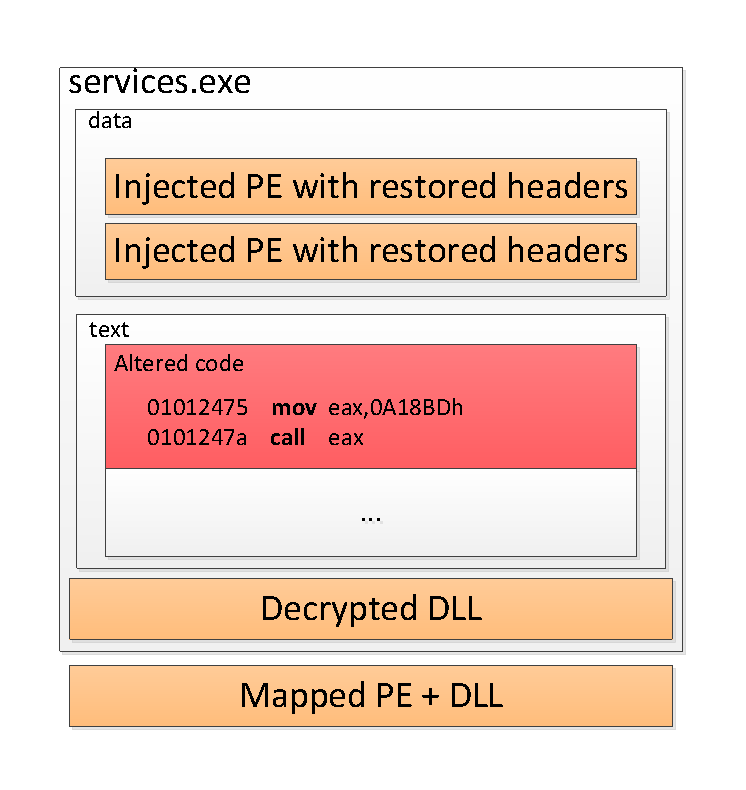
\includegraphics[width=0.4\textwidth]{img/injectionDuquMalware.pdf} 
\end{center}
\caption{Memory space injected by Duqu into services.exe once the injection is done.}
\label{fig:AThierry_ServiceMem}
\end{figure}



% il efface la zone a16c5 à a1703 pourquoi ???


The payload contained in the DLL is now in place and executed. Once it is done it sends a request to the driver through the access point $\backslash$\texttt{Device}$\backslash$\begin{small}\texttt{\{624409B3-4CEF-41c0-8B81-7634279A41E5\}}\end{small} so it restores the 12 first bytes located at the entrypoint of \service. A second request is finally sent to restore the access permission of \service's entrypoint.
% Lorsque le code injecté termine son action offensive, il envoie une première requête au driver à travers le point d'accès $\backslash$\texttt{Device}$\backslash$\texttt{\{624409B3-4CEF-41c0-8B81-7634279A41E5\}} afin que celui-ci modifie les droits d'accès de la page mémoire au point d'entrée de \service. Ainsi il peut rétablir les 12 octets préalablement sauvegardés par le driver pour lui dans la seconde structure (voir la figure \ref{fig:AThierry_InjectedDataStruct}). Il termine sa tâche par une seconde requête afin, cette fois-ci, de restaurer les droits d'accès d'origine.  

The injection is now done, control is then passed back to the restored \service.
% La mission de l'injection étant atteinte, l'exécution reprend son cours et cette fois-ci le processus \service\ original est exécuté.

\section{Turning the driver}
\label{section:utilisation}
%Un driver fonctionnel
%DUQU :
%détecte les nouveaux processus, quand service32 arrive il note son PID, détecte les DLL, quand kernel32 est utilisé, si le PID associé est celui de service32 il s'injecte dans la DLL
%Modifié :
%A chaque DLL injectée, on apprend un checksum du début de la fonction, si il y a un changement on lève une alerte (analyse AV par exemple)

% \subsection{Analyse fonctionnelle de la détection}
% \subsection{Analyse du driver}
In the previous paragraph we described how the \Duqu's DLL is injected in \service. Some of these mechanisms, for instance the notifications once a module is loaded, can be used for defensive purposes.
% Nous avons, dans la partie précédente, détaillé le déroulement de l'injection de la DLL de \Duqu\ dans \service. Certains de ces mécanismes, comme la mise en place de notifications lors du chargement en mémoire d'un binaire, peuvent clairement être utilisées à des fins défensives.

In a nutshell the modified driver will calculate signatures (checksums) on binaries upon notification that they are loaded into memory. On reception of further notifications, if the checksum has changed, an alert is risen and further actions might be taken.
% Schématiquement, le driver modifié calcule des signatures sur les binaires chargés en mémoire. Lorsqu'un binaire est lancé, dans le cas où sa signature n'est pas reconnue, un scan de la mémoire lui étant allouée est effectué, pouvant révéler la présence d'un malware.
Let's now go into some details of the initialization, memorization and detection phase of the defensive driver. We'll end this paper by a demonstration of the defense granted by the modified driver against an attack by \Duqu.
% Nous allons à présent détailler les phases d'initialisation, de mémorisation puis de détection du driver détourné. Nous terminerons ce papier par une présentation détaillée d'une exécution du binaire modifié en situation d'attaque par \Duqu.

\subsection{Initialization phase}

The initialization phase of our driver has been greatly simplified. We kept the creation of the access points, removed the search for the \texttt{ZwProtectVirtualMemory} function.
We kept the handling of notifications when modules are loaded and also asked for notifications when the system finishes creating a process (function \texttt{PsSetCreateProcessNotifyRoutine}).
% La phase d'initialisation de notre driver a été grandement allégée. Nous avons gardé la partie commune à tout driver à savoir la création des points d'accès (en prenant soin de les renommer) et supprimé la recherche de la fonction \texttt{ZwProtectVirtualMemory}. Par souci de simplification, les paramètres internes n'ont pas été chiffrés (chemin de la clé de registre \texttt{FILTER} et nom du device). Nous avons bien entendu conservé le système de notification des chargements de modules mais en plus nous lui avons ajouté une autre notification : lorsque le système termine la création d'un processus (fonction \texttt{PsSetCreateProcessNotifyRoutine}).
% (voir figure \ref{fig:WorkerRoutine}). 

% \begin{figure}
% \scriptsize
% % \begin{framed}
% \begin{changemargin}{-1cm}{-1cm}
% \begin{lstlisting}[language={C}]
% NTSTATUS WorkerRoutine(PDEVICE_OBJECT DeviceObject,PIO_WORKITEM IoWorkItem)
% {
% UNICODE_STRING routineName;
% 
%   IoFreeWorkItem(IoWorkItem);
% 
%   if (NULL == ZwQueryInformationProcess) {
%         RtlInitUnicodeString(&routineName, L"ZwQueryInformationProcess");
%         ZwQueryInformationProcess = (QUERY_INFO_PROCESS) MmGetSystemRoutineAddress(&routineName);
% 
%         if (NULL == ZwQueryInformationProcess) {
%             DbgPrint("Cannot resolve ZwQueryInformationProcess\n");
%         }
%   }
% 
%   if (NULL == ZwQueryInformationThread) {
%         RtlInitUnicodeString(&routineName, L"ZwQueryInformationThread");
%         ZwQueryInformationThread = (QUERY_INFO_THREAD) MmGetSystemRoutineAddress(&routineName);
% 
%         if (NULL == ZwQueryInformationThread) {
%             DbgPrint("Cannot resolve ZwQueryInformationThread\n");
%         }
%   }
% 
%   PsSetCreateProcessNotifyRoutine(CreateProcessNotify,FALSE);
%   return PsSetLoadImageNotifyRoutine(LoadImageNotifyRoutine);
% };
% \end{lstlisting}
% \end{changemargin}
% % \end{framed}
% \caption{Enregistrement des deux notifications.\label{fig:WorkerRoutine}}
% \end{figure}

\subsection{Memorization phase}
We saw that the alteration is not done when the first notification is triggered.
Thus, if a checksum had been done at that point, the modification of the entrypoint could be detected when the second notification is triggered.

% We detailed how \Duqu\ modifies the instructions of the entrypoint when \krn\ is loaded into memory.
% Thus, had a checksum been done when the first notification is triggered


% Thus a checksum could be done on the entrypoint before it is modified.
We reused \Duqu's checksum function which was originally called for obfuscating function names.
% Nous avons vu précédemment que \Duqu\ écrase le code du point d'entrée du service infecté uniquement à l'instant où \texttt{kernel32.dll} vient d'être mappée en mémoire. Nous avons donc tout le temps de réaliser une somme de contrôle à chaque point d'entrée avant son altération. Nous avons repris intégralement la fonction de hachage implémentée dans \Duqu\ et utilisée à l'origine pour retrouver le nom des fonctions de façon discrète.   

A first notification is received when a process is created. Unfortunately Windows passes only the process \texttt{id}, its parent and whether it was created or destroyed. However we can retrieve the PEB (Process Enviroment Block) structure associated to that process. We used that information to find the memory address of the loaded file.
% La première notification surviendra lorsqu'un nouveau processus sera créé par le système. Malheureusement pour nous, le système d'exploitation nous notifie uniquement l'\texttt{id} du processus, son parent et s'il vient d'être créé ou détruit. Cela dit, Windows peut nous fournir la structure PEB (Process Enviroment Block) associée au processus. Nous l'avons utilisée afin de déterminer l'adresse mémoire du fichier.


% (voir la figure \ref{fig:GetProcessInfos}).

% \begin{figure}[H]
% \scriptsize
% \begin{verbatim}
% NTSTATUS GetProcessInfos(HANDLE processId, PModuleInfosStuct pModuleStruct)
% {
%     NTSTATUS status;
%     ULONG returnedLength;
%     ULONG bufferLength;
%     HANDLE hProcess;
%     PEPROCESS eProcess;
%     PROCESS_BASIC_INFORMATION pbi;
%     PPEB pPEB;
%     PIMAGE_DATA_DIRECTORY EATAddr;
%     PVOID EntryPoint=NULL;
%     PKAPC_STATE ApcState;  
%     BOOLEAN result;
%     
%     PAGED_CODE(); // this eliminates the possibility of the IDLE Thread/Process
% 	
% 	status = PsLookupProcessByProcessId(processId, &eProcess);
% 
% 	if(NT_SUCCESS(status))
% 	{
% 		status = ObOpenObjectByPointer(eProcess,0, NULL, 0,0,KernelMode,&hProcess);
% 		if(NT_SUCCESS(status))
% 		{
% 		} else {
% 			DbgPrint("ObOpenObjectByPointer Failed: %08x\n", status);
% 		}
% 		ObDereferenceObject(eProcess);
% 	} else {
% 		DbgPrint("PsLookupProcessByProcessId Failed: %08x\n", status);
% 		return STATUS_UNSUCCESSFUL;
% 	}
% 	
% 	bufferLength = sizeof(PROCESS_BASIC_INFORMATION);
% 
%   
% 	ApcState = (PKAPC_STATE)ExAllocatePool(NonPagedPool, sizeof(KAPC_STATE));   
%         KeStackAttachProcess(eProcess, ApcState);   
% 
%         /* Retrieve the process path from the handle to the process */
%         status = ZwQueryInformationProcess( NtCurrentProcess(),
%                                         ProcessBasicInformation,
%                                         &pbi,
%                                         bufferLength,
%                                         &bufferLength);
% 
%         if (NT_SUCCESS(status)) 
% 	{
%         /* Copy the path name */
% 	   pPEB = pbi.PebBaseAddress;
% 	   pModuleStruct->ImageBaseAddr = pPEB->ImageBaseAddress;
%        
%            DbgPrint("ProcessImageInformation: PEB=0x%08x ImageBaseAddress=0x%08x UniqueProcessId=0x%x \n", 
%                        pPEB, pModuleStruct->ImageBaseAddr,pbi.UniqueProcessId);
%            
%            ParsePEModule(pModuleStruct);
% 	   
%            DbgPrint("ProcessImageInformation: Entrypoint=0x%08x DataDirectory=0x%08x \n", 
%                      pModuleStruct->Entrypoint, pModuleStruct->DataDirectory); 
%         }
% 	else {
%            DbgPrint("ProcessImageInformation failed: %x\n", status);
% 	}
% 	KeUnstackDetachProcess(ApcState);
% 
%     if ( hProcess )
%         ZwClose(hProcess);
% 
%     return status;
% }
% \end{verbatim}
% \caption{Identification de l'emplacement mémoire du fichier associé au processus.\label{fig:GetProcessInfos}}
% \end{figure}


% Pour une raison de simplification, nous allons nous focaliser uniquement sur l'infection du processus \service\ (visé par \Duqu).
% sans tenir compte qu'un autre processus peut être choisi comme cible (cela impliquerait la gestion d'une liste de tous les processus potentiellement ciblés). 
In order to detect \Duqu, we focused on \service, we compare the process name to the string "\service". If it is the target process, we look for its entrypoint, we calculate its hashed value and store it as an initial signature.
The defensive driver is now ready to detect the hook made by \Duqu.

% C'est pourquoi nous allons interroger le système afin de récupérer le nom du processus et de le comparer à la chaîne de caractères \service. Si le processus est identifié comme étant \service, nous procédons à la recherche de son point d'entrée% (voir la figure \ref{fig:ParsePEModule})
% , nous calculons son hash puis le sauvegardons comme valeur de référence. Nous sommes maintenant prêts à détecter la mise en place du \emph{hook} réalisé par \Duqu.


% \begin{figure}[H]
% \scriptsize
% \begin{verbatim}
% NTSTATUS __fastcall ParsePEModule(
%       __out PModuleInfosStuct pModuleStruct)
% {
%   PVOID infosPE; //IMAGE_NT_HEADER; 
%   PIMAGE_DOS_HEADER  pDosHeader     = NULL;
%   PIMAGE_NT_HEADERS  pNtHeader      = NULL;
%   PIMAGE_FILE_HEADER  pFileHeader   = NULL;
%   PIMAGE_OPTIONAL_HEADER32  pOptionHeader = NULL;
% 
%   infosPE=(PIMAGE_DOS_HEADER)pModuleStruct->ImageBaseAddr; 
%   if (((PIMAGE_DOS_HEADER)infosPE)->e_magic != 'ZM' )
%     return STATUS_WAIT_1;
% 
%   DbgPrint("  ParsePEModule: MZ\n");
% 
%   pNtHeader = (PIMAGE_NT_HEADERS32)((DWORD)infosPE + ((PIMAGE_DOS_HEADER)infosPE)->e_lfanew);
%   if ( (pNtHeader->Signature ^ 0xF750F284) != (IMAGE_NT_SIGNATURE ^ 0xF750F284)) 
%     return STATUS_WAIT_1; // 1
% 
%   DbgPrint("  ParsePEModule: PE\n");
% 
%   pFileHeader = (PIMAGE_FILE_HEADER)&pNtHeader->FileHeader;
%   pOptionHeader = (PIMAGE_OPTIONAL_HEADER32)&pNtHeader->OptionalHeader;
%   if ((pFileHeader->Machine ^ 0x594F) == (IMAGE_PE_i386_MACHINE ^ 0x594F)) 
%   {
%      DbgPrint("  ParsePEModule: Machine\n");
% 
%      if ((pOptionHeader->Magic ^ 0x5908) == (IMAGE_PE32_MAGIC ^ 0x5908) 
%           && (pFileHeader->SizeOfOptionalHeader == 0xE0 )) 
%      {
%           pModuleStruct->DataDirectory = 
%               (PIMAGE_DATA_DIRECTORY)&(pOptionHeader->DataDirectory[IMAGE_DIRECTORY_ENTRY_EXPORT]).VirtualAddress;  
% 	  pModuleStruct->Entrypoint = 
%               (PVOID)((DWORD)pModuleStruct->ImageBaseAddr + (DWORD)pOptionHeader->AddressOfEntryPoint);
%   	  pModuleStruct->EntrypointAddr = 
%               (DWORD)pModuleStruct->ImageBaseAddr + (DWORD)pOptionHeader->AddressOfEntryPoint;
%           pModuleStruct->EntrypointChecksum=
%               HashOfSectionName((BYTE *)pModuleStruct->EntrypointAddr);
%      
% 	  DbgPrint("  ParsePEModule: DataDirectory=0x%08x EntryPoint=0x%08x\n",
%                    pModuleStruct->DataDirectory,pModuleStruct->Entrypoint);
% 
% 	  return STATUS_SUCCESS; 
%      }
%   }
%   else if ((pFileHeader->Machine ^ 0xDE67) == (IMAGE_PE_x86_MACHINE ^ 0xDE67) 
%             && (pOptionHeader->Magic ^ 0x5A08) == (IMAGE_PE32_PLUS_MAGIC ^ 0x5A08) 
%             && pFileHeader->SizeOfOptionalHeader == 0xF0 ) // 64bits
%   {
% 	  DbgPrint("  ParsePEModule: Machine IMAGE_PE_x86_MACHINE\n");
% 
%           pModuleStruct->DataDirectory = 
%            (PIMAGE_DATA_DIRECTORY)&(pOptionHeader->DataDirectory[IMAGE_DIRECTORY_ENTRY_RESOURCE]).VirtualAddress; 
%           return STATUS_SUCCESS; 
%   }
%   return STATUS_WAIT_1;
% }
% \end{verbatim}
% \caption{Recherche du point d'entrée.}
% \label{fig:ParsePEModule}
% \end{figure}


\subsection{Detection phase}
When a module is loaded, the operating system passes control to the defensive driver which looks for the entrypoint of the module. If the loaded module is a DLL, the entrypoint is searched in the \texttt{PE} file of the executable file it is linked to.
We reused what was done in \Duqu\ and added the verification of the hash.

% Lorsque le système d'exploitation redonne la main à notre routine à la suite du chargement d'un module en mémoire, celle-ci commence par mémoriser l'adresse de base du module notifié puis l'utilise ensuite pour scruter l'entête du fichier \texttt{PE} à la recherche de son point d'entrée. Nous nous sommes contentés de reprendre ce qui a été fait dans \Duqu\ en ajoutant simplement le calcul de la somme de contrôle.


% (voir la Figure \ref{fig:ParsePEModule}). 
% Le hash pourrait être sauvegardé à ce niveau afin de permettre un contrôle d'intégrité sur l'ensemble des modules chargés en mémoire, nous nous sommes intéressés exclusivement au processus \service\ visé par \Duqu.

The hash of the PE file has been determined and is to be compared to the original signature previously stored.
If both checksums are different, we infer that \Duqu\ hooked \service\ between the two notifications. Since the entrypoint has been altered, the process \service\ is flagged as suspicious and submitted to further analysis.
% Passons au calcul du contrôle d'intégrité du processus surveillé (\service). Dans la phase précédente, nous avons sauvegardé son point d'entrée ainsi qu'un hash de référence. Nous procédons à un nouveau calcul de ce hash et le comparons à celui de référence. Si les deux hash sont différents, nous en déduisons que \Duqu\ a positionné son \emph{hook} entre deux notifications. Nous pouvons ainsi lire l'adresse cible du saut, procéder à un scan mémoire et analyser le code du processus ayant subi l'injection.    

\subsection{Proof of concept}
Aiming to debug and test the original driver and the defensive one, we followed the steps described by Sergei Shevchenko \cite{FSabatier_SShevchenko} who proposes to rename the Windows calculator \texttt{calc.exe} as \service\ and launch it to watch how the drivers react.

For this example we used two virtual machines using \texttt{Windows XPSP3} connected by a serial link. The first machine runs Microsoft's \texttt{WinDBG} for kernel debug. The other machine is launched in \texttt{"kernel debug"} mode which allows the debug machine to communicate on a kernel level and debug drivers.

While doing tests we uncovered that \Duqu's \texttt{nfrd965.sys} checks if the system is in debug or failsafe mode so we had to patch that out for test purposes, thus allowing debug.
We also configured both drivers so they can be launched on demand, it was needed to modify registry keys (the \texttt{Start} parameter has to be set to 3).
This configuration provides us with the possibility to choose the launch order of both drivers and \service.

% Lors de cette démonstration nous utilisons deux machines virtuelles sous \texttt{Windows XPSP3} reliées par un cable série lui aussi virtuel. Sur la première machine, nous lançons le débogueur de Microsoft \texttt{WinDBG} en mode \texttt{kernel} écoutant sur le port \texttt{COM2}. Sur la seconde, le système est démarré en mode \texttt{"kernel debug"}. Cette configuration nous permettra de lancer notre driver de détection puis le driver \texttt{nfrd965.sys} de \Duqu\space ou inversement.

% Pour faciliter la mise au point de ce driver de détection, nous l'avons installé manuellement sur une machine de test ainsi que celui de \Duqu\space en nous inspirant fortement de la démarche proposée par Sergei Shevchenko \cite{FSabatier_SShevchenko}. Ainsi lorsque nous ouvrons la calculatrice renommée en \service , notre driver entre en action.

% Cependant, lors de la reconstitution du code source, nous avons remarqué que le driver \texttt{nfrd965.sys} vérifie que le système n'est ni en mode sans échec, ni en mode débogage (Figure \ref{fig:AThierry_AntiDebug}).

% \begin{figure*}
% \scriptsize
% % \begin{framed}
% \begin{lstlisting}[language={C}]
%      if(status == STATUS_SUCCESS) {
%         decode_parameters(RegistryPath);
%         if ( ((ULONG)&g_DefaultParamCrypted & 1) && *InitSafeBootMode != 0) {
%                     status = STATUS_UNSUCCESSFUL;
%         } else if ( ((ULONG)&g_DefaultParamCrypted & 2)) {
%                  if (*KdDebuggerEnabled ==0 ) {
%                       status = STATUS_UNSUCCESSFUL;
%                  } else {
%                       status = STATUS_SUCCESS;
%                  }
%         } else {
%                  status = STATUS_SUCCESS;
%         }
% \end{lstlisting}
% 
% % \end{framed}
% 
% \caption{Détection du mode sans échec, ainsi que le mode débogage.\label{fig:AThierry_AntiDebug}}
% \end{figure*}


% Pour retirer cette restriction nous avons patché le driver comme le montre la Figure \ref{fig:AThierry_patch} : on remplace simplement un saut conditionnel \emph{jz} par un saut inconditionnel \emph{jmp}. Nous copions ce driver ainsi patché dans le répertoire \texttt{C}$\backslash$\texttt{WINDOWS}$\backslash$\texttt{system32}$\backslash$\texttt{drivers}$\backslash$ ainsi que la DLL chiffrée à l'aide de la routine extraite du code source dans le répertoire \texttt{C}$\backslash$\texttt{WINDOWS}$\backslash$\texttt{inf}$\backslash$ sous le nom \netpDLL. Il nous reste à configurer les clés de registre renfermant les paramètres utilisés par le driver lors de son initialisation.
% Les valeurs remarquables sont le nom du driver (\texttt{DisplayName=nfrd965}), son groupe (\texttt{Group=Network}), son emplacement (\texttt{ImagePath}=C:\textbackslash WINDOWS\textbackslash System32 \textbackslash Drivers\textbackslash nfrd965.sys), la valeur de ses paramètres internes (repris de \texttt{Crysys}) et les paramètres de démarrage (\texttt{Start=3} et \texttt{Type=1}).
% L'attribut \texttt{Type} indique qu'il s'agit d'un driver du noyau pour un appareil (ici de type \texttt{Network}), l'attribut \texttt{Start} spécifie le moment de lancement du driver : nous l'avons positionné à 3 (lancement à la demande) pour nous permettre de démarrer le driver défensif avant ou après celui de \Duqu.


% (voir la figure \ref{fig:registry}).

% \begin{figure*}
% \begin{center}
% %\begin{changemargin}{-2cm}{-2cm}
% \includegraphics[width=0.8\textwidth]{img/patch.pdf}
% %\end{changemargin}
% \caption{Patch de la détection du mode débogage.}
% \label{fig:AThierry_patch}
% \end{center}
% \end{figure*}

% \begin{figure}
% \begin{center}
%  \includegraphics[width=1.0\textwidth]{AThierry/img/registry.pdf}
% \end{center}
% \caption{Définition des clés de registre.}
% \label{fig:registry}
% \end{figure}


% Lors de cette démonstration nous utilisons deux machines virtuelles sous \texttt{Windows XPSP3} reliées par un cable série lui aussi virtuel. Sur la première machine, nous lançons le débogueur de Microsoft \texttt{WinDBG} en mode \texttt{kernel} écoutant sur le port \texttt{COM2}. Sur la seconde, le système est démarré en mode \texttt{"kernel debug"}. Cette configuration nous permettra de lancer notre driver de détection puis le driver \texttt{nfrd965.sys} de \Duqu\space ou inversement.

We first launched the defensive driver, then \Duqu's driver and finally \service.
In the debugger console, shown on Figure  \ref{fig:AThierry_Breakpoint1}, we see when \service\ is launched. The system notifies the defensive driver which outputs information about the loaded module then stores its \texttt{id}, the address of its entrypoint and its initial signature (checksum of the first bytes at the entrypoint).

% En regardant de près la fenêtre de commandes du débogueur, nous constatons le chargement en mémoire du driver de \Duqu\ car le système a envoyé une notification à notre driver à la fin de sa tâche (voir la Figure \ref{fig:AThierry_LaunchNFRD965}). 
% \begin{figure*}
% \scriptsize
% Microsoft (R) Windows Debugger Version 6.12.0002.633 X86
% Copyright (c) Microsoft Corporation. All rights reserved.
% 
% Opened \\.\COM2
% Waiting to reconnect...
% Connected to Windows XP 2600 x86 compatible target at (Fri Jan 18 14:55:17.808 2013 (UTC + 1:00)), ptr64 FALSE
% Kernel Debugger connection established.
% Symbol search path is: SRV*c:\windows\symbols*http://msdl.microsoft.com/download/symbols
% Executable search path is: 
% Windows XP Kernel Version 2600 UP Free x86 compatible
% Built by: 2600.xpsp_sp3_gdr.101209-1647
% Machine Name:
% Kernel base = 0x804d7000 PsLoadedModuleList = 0x805540c0
% System Uptime: not available
% Break instruction exception - code 80000003 (first chance)
% *******************************************************************************
% *                                                                             *
% *   You are seeing this message because you pressed either                    *
% *       CTRL+C (if you run kd.exe) or,                                        *
% *       CTRL+BREAK (if you run WinDBG),                                       *
% *   on your debugger machine's keyboard.                                      *
% *                                                                             *
% *                   THIS IS NOT A BUG OR A SYSTEM CRASH                       *
% *                                                                             *
% * If you did not intend to break into the debugger, press the "g" key, then   *
% * press the "Enter" key now.  This message might immediately reappear.  If it *
% * does, press "g" and "Enter" again.                                          *
% *                                                                             *
% *******************************************************************************
% 
% [...]

% \begin{lstlisting}[language={}]
% --** Load driver \??\c:\WINDOWS\system32\drivers\nfrd965.sys **--
% LoadImageNotifyRoutine: ImageBaseAddress=0xf78c5000 ProcessId=0x0 
%   ParsePEModule: MZ
%   ParsePEModule: PE
%   ParsePEModule: Machine
% Entrypoint bytes at 0xf78c5570: 0x55 0x8b 0xec 0x6a 0xff 0x68 0x08 0xa1
%   ParsePEModule: DataDirectory=0xf78c5160 EntryPoint=0xf78c5570
% LoadImageNotifyRoutine: Entrypoint=0xf78c5570 DataDirectory=0xf78c5160 
% \end{lstlisting}
% \caption{Exécution du driver nfrd965.sys. La routine \texttt{LoadImageNotifyRoutine} de notre driver nous le signale.\label{fig:AThierry_LaunchNFRD965}}
% \end{figure*}

% Pour déterminer plus facilement le moment où intervient notre driver, nous décidons de positionner deux points d'arrêt dans le driver \Duqu\ . Le premier, au moment où il sauvegarde les octets du point d'entrée et le second au moment où il exécute le code du module tremplin. 
% Nous pouvons dès lors lancer \service\ : la réaction est immédiate (voir la figure \ref{fig:AThierry_Breakpoint1}).  

\begin{figure}
% \begin{changemargin}{-2cm}{-2cm}
% \begin{center}
%  \includegraphics[width=1.0\textwidth]{AThierry/img/bw-breakpoint1.pdf}
% \end{center}
% \end{changemargin}

% ----------+++++++++****** Create process 0x914 *******+++++++++-----------
% ProcessImageInformation: PEB=0x7ffd6000 ImageBaseAddress=0x01000000 UniqueProcessId=0x914 
% Entrypoint bytes at 0x01012475: 0x6a 0x70 0x68 0xe0 0x15 0x00 0x01 0xe8
%   ParsePEModule: DataDirectory=0x01000168 EntryPoint=0x01012475
% ProcessImageInformation: Entrypoint=0x01012475 DataDirectory=0x01000168 
% ProcessImageName: \Device\HarddiskVolume1\Documents and Settings\fabrice\Bureau\services.exe
% ======= ProcessImageName: save processID=0x914
% CreateProcessNotify: ImageBaseAddress=0x01000000 EntryPoint=0x01012475 
% CreateProcessNotify: Create=1 0x788=>0x914
% CreateProcessNotify: EntrypointChecksum=0x49af1bf2
% --** Load module \Device\HarddiskVolume1\Documents and Settings\fabrice\Bureau\services.exe **--
% LoadImageNotifyRoutine: ImageBaseAddress=0x01000000 ProcessId=0x914 
% Entrypoint bytes at 0x01012475: 0x6a 0x70 0x68 0xe0 0x15 0x00 0x01 0xe8
%   ParsePEModule: DataDirectory=0x01000168 EntryPoint=0x01012475
% LoadImageNotifyRoutine: Entrypoint=0x01012475 DataDirectory=0x01000168 
% ------>>> Verify services.exe processus: Entrypoint bytes at 0x01012475: 0x6a 0x70 0x68 0xe0 0x15 0x00 0x01 0xe8
%  OK! 
\scriptsize
\begin{lstlisting}[language={}]
-+* Create process 0x914 *+-
ProcessImageInformation: 
  PEB=0x7ffd6000 ImageBaseAddress=0x01000000
  UniqueProcessId=0x914 
Entrypoint bytes at 0x01012475: 
  0x6a 0x70 0x68 0xe0 0x15 0x00 0x01 0xe8
ProcessImageName: Desktop\services.exe
ProcessImageName: save processID=0x914
CreateProcessNotify: ImageBaseAddress=0x01000000
  EntryPoint=0x01012475
  EntrypointChecksum=0x49af1bf2
\end{lstlisting}
\caption{From WinDbg: The process services.exe is loaded. The defensive driver stores its id (\texttt{0x914}), its entrypoint (\texttt{0x01012475}) and its hash (\texttt{0x49af1bf2}).\label{fig:AThierry_Breakpoint1}}
\end{figure}

% La logique voudrait que le système commence par charger le fichier \service\ en mémoire puis crée un processus du même nom. Mais on constate que notre driver reçoit les notifications dans l'ordre inverse. Heureusement cela n'a pas d'impact sur notre méthode de détection. Ainsi lors de la création du processus, nous sauvegardons son \texttt{id}, son point d'entrée et calculons la somme de contrôle qui servira de signature.  
When the notification for \krn\ is triggered to the defensive driver, no modification has been made since \Duqu's driver will receive the notification afterwards (due to the launch order of drivers). So the checksum succeeds. However there are further notifications, for instance when the linked DLL \texttt{shell32.dll} is loaded, the defensive driver checks once again the entrypoint's hash and it has been altered. It is shown on Figure \ref{fig:AThierry_Breakpoint2}. Thus the alteration of \service\ is detected and the defensive driver takes further steps to protect the system: it terminates \service, ending \Duqu's attempt to compromise the machine.
% Nous poursuivons son exécution et arrivons à l'instant où le système charge la DLL \krn\ en mémoire et par conséquence notifie le driver \texttt{nfrd965.sys} (voir la Figure \ref{fig:AThierry_Breakpoint2}).

\begin{figure}
% \begin{changemargin}{-2cm}{-2cm}
% \begin{center}
%  \includegraphics[width=1.1\textwidth]{AThierry/img/bw-breakpoint2.pdf}
% \end{center}
% \end{changemargin}
\scriptsize
% \begin{framed}
\begin{lstlisting}[language={}]
* Loaded module \WINDOWS\system32\kernel32.dll *
LoadImageNotifyRoutine:
  ImageBaseAddress=0x7c800000 ProcessId=0x914 
-> Verify services.exe process: 
   Entrypoint at 0x01012475:
     0x6a 0x70 0x68 0xe0 0x15 0x00 0x01 0xe8
-> OK!
* Loaded module \WINDOWS\system32\shell32.dll *
LoadImageNotifyRoutine:
  ImageBaseAddress=0x7c9d0000 ProcessId=0x914 
-> Verify services.exe process:
   Entrypoint at 0x01012475:
     0xb8 0xbd 0x18 0x0a 0x00 0xff 0xd0 0xe8
-> Checksum error !!!!
-> Terminating services.exe
\end{lstlisting}
% \end{framed}
\caption{Detection of the altered entrypoint (\texttt{0x01012475}) of services.exe.\label{fig:AThierry_Breakpoint2}}
\end{figure}

% Lorsque notre driver est démarré avant le driver \texttt{nfrd965.sys}, nous recevons la notification de chargement de module avant lui. Ainsi lorsque la DLL \texttt{kernel32.dll} est notifiée à notre driver, \Duqu\ n'a pas encore altéré le point d'entrée. C'est pourquoi la somme de contrôle est toujours correcte (cela n'aurait pas été le cas si \Duqu\ avait démarré avant le notre). Par contre, au chargement de la DLL suivante (\texttt{shell32.dll}), nous détectons la modification du point d'entrée. Cette modification est déjà suspecte et pourrait justifier l'arrêt du processus \service\ mais nous voulons être capable de retrouver la similarité avec \Stuxnet\ trouvée dans leurs DLLs.
% Une analyse manuelle du code injecté dans \service\ révèle que la DLL de \Duqu\ est chargée à l'adresse \texttt{0xb0028}. Afin de retrouver automatiquement cette DLL, on peut tenter de suivre le code injecté (par analyse statique), scanner les pages mémoires allouées par \service\ ou scanner l'ensemble de la mémoire à la recherche d'images exécutables. Pour l'instant le driver se contente de scanner l'adresse trouvée à la main.

% Nous connaissons à présent l'adresse où est situé le code injecté par \Duqu\ dans \service.
% (voir la figure \ref{fig:hook})
% Le driver réalise alors le dump de cette DLL inconnue et, connaissant \Stuxnet, un scan lève une alerte : elle présente des similarités avec ce dernier. Le driver met alors fin au processus utilisant la DLL (\service).

% Notre méthode de détection fonctionne par comparaison des graphes des flot de contrôle (CFG) \cite{AThierry_BKM08}, plus de détails sur cette technique de détection et son application à \Duqu\ et \Stuxnet\ ont été donnés dans de précédents travaux \cite{AThierry_REAT12,AThierry_MAL12}.

% \begin{figure}
% \scriptsize
% % \begin{framed}
% \begin{verbatim}
% 0x01012475    b8 bd 18 0a 00   mov eax,0A18BDh 
% 0x0101247a    ff d0            call eax
% \end{verbatim}
% % \end{framed}
% \caption{Saut sur le code injecté dans \texttt{\service}.\label{fig:hook}}
% \end{figure}

\section{Conclusion}
Similarities between \Duqu\ and \Stuxnet\ lead us to look for a detection method of \Duqu\ when the attack is going on.
We described by and large the infection technique of \Duqu\ and how its driver operates, stealthy injecting code into \service\ using kernel functions.
Thus we rebuilt a source code for \Duqu's driver and created a defensive version from this source code. Our modified driver is able to detect the injection made by \Duqu\ and protects the system by terminating the infected process \service.

% Let us do one step behind. 
\Duqu\ was considered at its times as one of the most sophisticated malware. And the above shows that, indeed, the malware was built with great care. At the same time, it is known that complex systems may be fragile. Usually, it is on the defender side that we make the observation: complex infrastructures offer a lot of entry points to malware. Here, the argument is opposite: it's the malware which was fragile and we exploited this feature to turn it for our own purposes.
% For once.


% Les similarités entre \Duqu\ et \Stuxnet\ nous ont poussé à chercher une technique capable de détecter \Duqu\ dans une situation d'attaque. À partir de la DLL principale de \Stuxnet\ nous reconnaissions celle de \Duqu\ mais encore fallait-il avoir accès à celle-ci une fois déchiffrée.
% Nous avons détaillé la technique d'infection de \Duqu\ et le fonctionnement de son driver, capable d'injecter discrètement du code dans \service\ à l'aide de routines du noyau.
% Nous avons donc reconstruit le code source de ce dernier et l'avons détourné à des fins défensives. Utilisé pour intercepter les chargement de binaires par le système d'exploitation et interfacé avec notre détecteur, le driver a été capable de détecter l'injection effectuée par \Duqu.
% Il est de plus possible de classer l'attaque comme liée à \Stuxnet\ à condition de fournir l'adresse où est présente la DLL injectée en mémoire.

% Dans la suite nous allons chercher à récupére\sqsubseteq\sqsubseteq\sqsubseteq\sqsubseteq\sqsubseteq\sqsubseteq\sqsubseteq\sqsubseteq\sqsubseteq\sqsubseteq\sqsubseteq\sqsubseteq\sqsubseteq\sqsubseteq\sqsubseteq\sqsubseteq\sqsubseteq\sqsubseteq\sqsubseteq\sqsubseteq\sqsubseteq\vartriangleright\vartriangleright\vartrianglerightr cette adresse automatiquement pour éviter d'avoir à scanner l'intégralité de la mémoire.



%
%\bibliographystyle{unsrt}
%\bibliographystyle{ieeetr}
~\\
\bibliographystyle{latex8} 
% \nocite{*}
\bibliography{malware2013}


\end{document}
%%% Local Variables:
%%% mode: TeX-PDF
%%% TeX-master: "master"
%%% End:
